\documentclass[twocolumn,twoside,letterpaper]{article} 

\usepackage{color}

\usepackage{geneticsT2}
\usepackage{times}
\usepackage{hyperref}

\addtolength{\oddsidemargin}{-.2cm}
\addtolength{\evensidemargin}{-1.2cm}

\addtolength{\textwidth}{1.5cm}
\addtolength{\topmargin}{-2cm}
\addtolength{\textheight}{3.5cm}

\renewcommand{\textfraction}{0.01}
\renewcommand{\topfraction}{0.99}
\renewcommand{\bottomfraction}{0.65}
\renewcommand{\floatpagefraction}{0.90}
\renewcommand{\dbltopfraction}{0.95}
\renewcommand{\dblfloatpagefraction}{0.80}
\renewcommand{\sfdefault}{phv}

% plr added
\usepackage{amsmath}
\usepackage{amssymb}
\newcommand{\E}{\mathbb{E}}
\renewcommand{\P}{\mathbb{P}}
\newcommand{\var}{\mathop{\mbox{Var}}}
\newcommand{\mutrate}{\lambda_{\text{mut}}}
\newcommand{\migrate}{\lambda_{\text{mig}}}
\newcommand{\Tmut}{T_{\text{mut}}}
\newcommand{\Tmig}{T_{\text{mig}}}


\usepackage{fancyhdr}
\pagestyle{fancy}
\fancyhf{}

\fancyfoot[LE,RO]{{\sfbf \thepage}}
\renewcommand{\headrulewidth}{0pt}
\fancypagestyle{plain}{
	\fancyhf{}
}

%editing commands (please leave in for now)
\newcommand{\jri}[1]{\textcolor{blue}{ \emph{\scriptsize  #1}} }
\newcommand{\st}[1]{\textcolor{red}{#1}}
\newcommand{\comst}[1]{\textcolor{red}{ \em{\scriptsize  #1}} }
\definecolor{mattgreen} {rgb} {0,0.6,0}
\newcommand{\mbh}[1]{\textcolor{mattgreen}{ \em{\scriptsize  #1}} }
\definecolor{peterpurple}{rgb}{.6,0,.6}
\newcommand{\plr}[1]{\textcolor{peterpurple}{ \emph{\scriptsize (#1)}} }

\usepackage[normalem]{ulem}
\def\dt{\bgroup
 \markoverwith{\lower-0.2ex\hbox
 {\kern-.03em\vbox{\hrule width.2em\kern0.45ex\hrule}\kern-.03em}}%
 \ULon}
\MakeRobust\dt
\usepackage[normalem]{ulem}
\def\dt{\bgroup
 \markoverwith{\lower-0.2ex\hbox
 {\kern-.03em\vbox{\hrule width.2em\kern0.45ex\hrule}\kern-.03em}}%
 \ULon}
\MakeRobust\dt

%%%%

\title{Independent adaptation to high elevation in maize}
\author{
 \small\sfbf{Shohei Takuno$^{\ast}$, Peter Ralph$^{\dag, \ddag}$, Sofiane Mezmouk$^{\ast}$, Kelly Swarts$^{\S}$, Rob J. Elshire$^{\S}$, Jeffrey C. Glaubitz$^{\S}$,}\\
   \small\sfbf{Edward S. Buckler$^{\S, \ast\ast}$, Matthew B. Hufford$^{\ast, \dag\dag}$, and Jeffrey Ross-Ibarra$^{\ast,\ddag\ddag,}$}\thanks{
Corresponding author:  Department of Plant Sciences, University of California, Davis, California 95616, USA. 
    E-mail: \mbox{rossibarra@ucdavis.edu}}\\[0.3cm]
   \small\sf $^{\ast}$Department of Plant Sciences, University of California, Davis, California 95616, USA,\\
   \small\sf $^\dag$Department of Evolution and Ecology, University of California, Davis, California 95616, USA,\\
   \small\sf $^\ddag$Molecular and Computational Biology, University of Southern California,  Los Angeles,California 90089-0371, USA,\\
   \small\sf $^\S$Institute for Genomic Diversity, Cornell University, Ithaca, New York 14853-2703, USA,\\
   \small\sf $^{\ast\ast}$US Department of Agriculture -- Agriculture Research Service (USDA-ARS) \st{address},\\
   \small\sf $^{\dag\dag}$Department of Ecology, Evolution, and Organismal Biology, Iowa State University, Ames, Iowa 50011, USA,\\
   \small\sf $^{\ddag\ddag}$The Center for Population Biology and the Genome Center, University of California, Davis, California 95616 , USA\\
}

 
\date{Revised manuscript for \emph{Genetics}, \today}

\abstract{
Repeated evolutions occurs when multiple species/subpopulations adapt to similar environments via mutations in the same locus. \jri{we define this more broadly in the intro.}
We investigate here the molecular basis of maize adaptation to highland climates in Mexico and South America using genome-wide SNP data. 
Taking advantage of archaeological data on the arrival of maize to the highlands, we infer demographic models for both populations, identifying evidence of a strong bottleneck and rapid expansion in South America.  
We use these models to then identify loci showing an excess of differentiation as a means of identifying putative targets of natural selection, and compare our results to expectations from recently developed theory on parallel adaptation.  
In spite of similar morphologies, we see limited evidence of selection on quantitative traits, and, consistent with predictions across a wide array of parameter space, we see few SNPs showing signs of parallel adaptation.
Instead, we show that selection appears to have predominantly acted on standing genetic variation, and that introgression from wild teosinte populations appears to have played a role in adaptation in Mexican maize.
We discuss the significance of these results in the context of the molecular basis of adaptation to new environments. \jri{abstract could use some more exciting wording }}

\usepackage{natbib}
\bibpunct{(}{)}{;}{a}{}{,}

\usepackage{amsmath}

\usepackage{graphicx}

\begin{document}

\maketitle

%%%%%%%%%%%%%%%%%%%%%%%%%%%%%%%%%%%%%%%%%% INTRO
\section*{Introduction}
\noindent Convergent evolution occurs when multiple species or populations exhibit similar phenotypic adaptations to comparable environmental challenges \cite[]{Wood_2005_15881688,Arendt_2008_18022278,Elmer_2011_21459472}.
Evolutionary genetic analysis of a wide range of species has provided evidence for multiple pathways of convergent evolution. 
One such route occurs when identical mutations arise independently and fix via natural selection in multiple populations. 
In humans, for example, malaria resistance due to mutations from Glu to Val at the sixth codon of the $\beta$-globin gene has arisen independently on multiple unique haplotypes  \cite[]{Currat_2002_11741197,Kwiatkowski_2005_16001361}.  
Convergent evolution can also be achieved when different mutations arise within the same locus yet produce similar phenotypic effects.  
Grain fragrance in rice appears to have evolved along these lines, as populations across East Asia have similar fragrances resulting from at least eight distinct loss-of-function alleles in the  \emph{BADH2} gene \cite[]{Kovach_2009_19706531}.  
Finally, convergent evolution may arise from natural selection acting on standing genetic variation in an ancestral population.  
In the three-spined stickleback, natural selection has repeatedly acted to reduce armor plating in independent colonizations of freshwater environments.  
Adaptation in these populations occurred both from new mutations as well as standing variation at the \emph{Eda} locus in marine populations \cite[]{Colosimo_2005_15790847}.  

Not all convergent phenotypic evolution is the result of convergent evolution at the molecular level, however.  
Recent studies of adaptation to high elevation in humans, for example, reveal that the genes involved in highland adaptation are largely distinct among Tibetan, Andean and Ethiopian populations \cite[]{Bigham_2010_20838600,Scheinfeldt_2012_22264333,Alkorta-Aranburu_2012_23236293}. 
While observations of independent origin may be due to a complex genetic architecture or standing genetic variation, introgression from related populations may also play a role.  
In Tibetan populations, the adaptive allele at the \emph{EPAS1} locus appears to have arisen via introgression from Denisovans, a related hominid group \cite[]{huerta2014altitude}.
Overall, we still know relatively little about how convergent phenotypic evolution is driven by common genetic changes or the relative frequencies of these different routes of convergent evolution.

The adaptation of maize to high elevation environments (\emph{Zea mays} ssp. \emph{mays}) provides an excellent opportunity to investigate the molecular basis of convergent evolution.  
Maize was domesticated from the wild teosinte \emph{Zea mays} ssp. \emph{parviglumis} (hereafter \emph{parviglumis}) in the lowlands of southwest Mexico $\sim$9,000 years before present (BP) \cite[]{Matsuoka_2002_11983901,Piperno_2009_19307570,vanHeerwaarden_2011_21189301}. 
After domestication, maize spread rapidly across the Americas, reaching the lowlands of South America and the high elevations of the Mexican Central Plateau by $\sim 6,000$ BP \cite[]{Piperno_2006_69}, and the Andean highlands by $\sim 4,000$ BP \cite[]{Perry_2006_16511492,Grobman_2012_22307642}. 
The transition from lowland to highland habitats spanned similar environmental gradients in Mesoamerica and S. America (Figure~\ref{supp:colfreq}) and presented a host of novel challenges that often accompany highland adaptation including reduced temperature, increased ultraviolet radiation, and reduced partial pressure of atmospheric gases \cite[]{Korner_2007_17988759}.

Common garden experiments in Mexico reveal that highland maize has successfully adapted to high elevation conditions \cite[]{Mercer2008}, and phenotypic comparisons between Mesoamerican and S. American populations are suggestive of convergent evolution.  
Maize landraces (open-pollinated traditional varieties) from both populations share a number of phenotypes not found in lowland populations, including dense macrohairs \cite[]{Wilkes_1977,Wellhausen1957:book}, stem pigmentation \cite[]{Wilkes_1977,Wellhausen1957:book}, differences in tassel branch and ear husk number \cite[]{brewbaker2014diversity}, and biochemical response to UV radiation \cite[]{Casati2005}. 
In spite of these shared phenotypes, genetic analyses of maize landraces from across the Americas indicate that the two highland populations are independently derived from their respective lowland populations \cite[]{Vigouroux_2008_21632329, vanHeerwaarden_2011_21189301}, suggesting that observed patterns of phenotypic similarity are not simply due to recent shared ancestry. 

In addition to convergent evolution between maize landraces, a number of lines of evidence suggest convergent evolution in the related wild teosintes.  
\emph{Zea mays} ssp. \emph{mexicana} (hereafter \emph{mexicana}) is native to the highlands of central Mexico, where it is thought to have occurred since at least the last glacial maximum \cite[]{Ross-Ibarra_2009_19153259, Hufford_niche}. 
Phenotypic differences between \emph{mexicana} and the lowland \emph{parviglumis} mirror those between highland and lowland maize \cite[]{Lauter_2004_15342532}, and population genetic analyses of the two subspecies reveal evidence of natural selection associated with altitudinal differences between \emph{mexicana} and \emph{parviglumis} \cite[]{Pyhajarvi2013,fang2012megabase}.  
Landraces in the highlands of Mexico are often found in sympatry with \emph{mexicana} and gene flow from \emph{mexicana} likely contributed to maize adaptation to the highlands \cite[]{Profford_2013}. 
No wild \emph{Zea} occur in S. America, and S. American landraces show no evidence of gene flow from Mexican teosinte \cite[]{vanHeerwaarden_2011_21189301}, 
further suggesting independent origins for altitude-adapted traits.

Here we use genome-wide SNP data from Mesoamerican and S. American landraces to investigate the evidence for convergent evolution to highland environments at the molecular level.  
We estimate demographic histories for maize in the highlands of Mesoamerica and S. America, then use these models to identify loci that may have been the target of selection in each population.
We find a large number of sites showing evidence of selection, consistent with a complex genetic architecture involving many phenotypes and numerous loci.  
We see little evidence for shared selection at the nucleotide or gene level, a result we show is consistent with expectations from recent theoretical work on convergent adaptation \cite[]{ralph2014convergent}.
Instead, our results support a role of adaptive introgression from teosinte in Mexico and highlight the contribution of standing variation to adaptation in both populations.

%%%%%%%%%%%%%%%%%%%%%%%%%%%%%%%%%%%%%%%%%% INTRO


%%%%%%%%%%%%%%%%%%%%%%%%%%%%%%%%%%%%%%%%% FIGURE
\begin{figure*}[tb]   
  \begin{center}
   \vspace{-0mm}
   %\includegraphics[width=0.23\textwidth]{figs/model}
   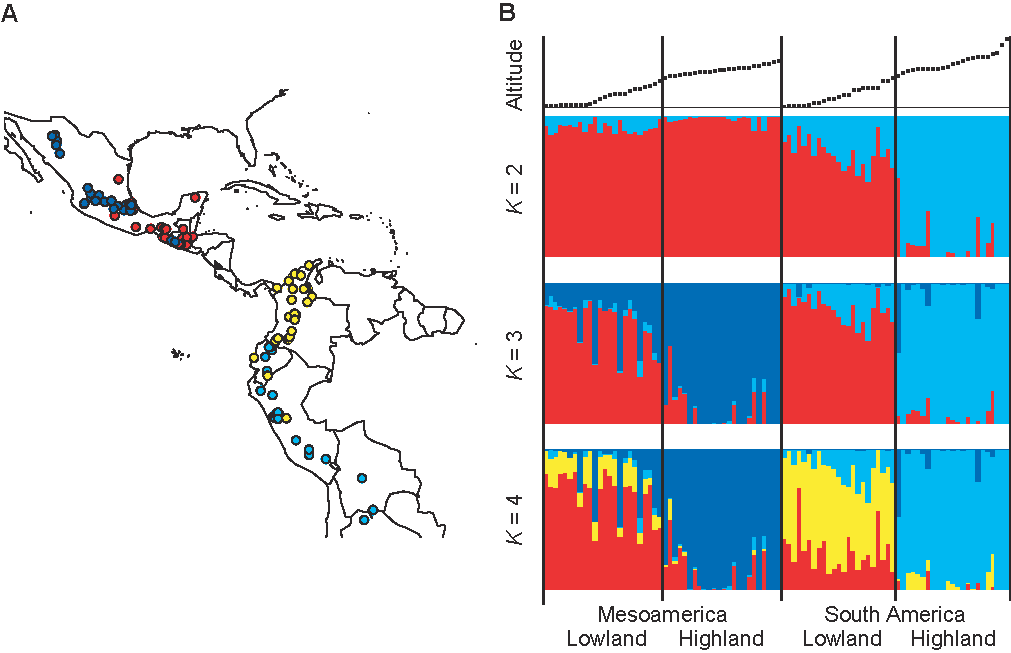
\includegraphics[width=0.8\textwidth]{fig/Fig2}
   \renewcommand{\baselinestretch}{0.9}
   \vspace{-3mm}
   \caption{(A) Sampling locations of landraces.  Red, blue, yellow and light blue dots represent Mexican lowland, Mexican highland, S. American lowland and S. American highland populations, respectively.  (B) Results of {\sf STRUCTURE} analysis of the maizeSNP50 SNPs with $K=2\sim4$.  The top panel shows the elevation, ranging from 0 to 4,000 m on the \emph{y}-axes.  The colors in $K=4$ correspond to those in panel (A).    }
\vspace{-6mm}
    \label{map}
  \end{center}
\end{figure*}
%%%%%%%%%%%%%%%%%%%%%%%%%%%%%%%%%%%%%%%%% FIGURE

\section*{Materials and Methods}

\subsection*{Materials and DNA extraction}
We included one individual from each of 94 open-pollinated landrace maize accessions from high and low elevation sites in Mexico and S. America (Table \ref{srkid}).   
Accessions were provided by the USDA germplasm repository or kindly donated by Major Goodman (North Carolina State University).  
Sampling locations are shown in Figure~\ref{map}A.  
Landraces sampled from elevations $<1,700$ m were considered lowland, while accessions from $>1,700$ m were considered highland.  
Seeds were germinated on filter paper following fungicide treatment and grown in standard potting mix.  
Leaf tips were harvested from plants at the five leaf stage.  
Following storage at $-80^{\circ}$C overnight, leaf tips were lyophilized for 48 hours.  
Tissue was then homogenized with a Mini-Beadbeater-8 (BioSpec Products, Inc., Bartlesville, OK, USA).  
DNA was extracted using a modified CTAB protocol \cite[]{CTAB}.  
The quality of DNA was ensured through inspection on a 2\% agarose gel and quantification of the ratio of light absorbance at 260 and 280 nm using a NanoDrop spectrophotometer (Thermo Scientific, NanoDrop Products, Wilmington, DE, USA).

\subsection*{SNP data}
We generated two complementary SNP data sets for the sampled maize landraces. 
The first set was generated using the Illumina MaizeSNP50 BeadChip platform, including 56,110 SNPs \cite[]{Ganal_2011_22174790}.  
SNPs were clustered with the default algorithm of the GenomeStudio Genotyping Module v1.0 (Illumina Inc., San Diego, CA, USA) and then visually inspected and manually adjusted.   
These data are referred to as "MaizeSNP50" hereafter.  
This array contains SNPs discovered in multiple ascertainment schemes \cite[]{Ganal_2011_22174790}, but the vast majority of SNPs come from polymorphisms distinguishing the maize inbred lines B73 and Mo17 (14,810 SNPs) or identified from sequencing 25 diverse maize inbred lines \cite[40,594 SNPs;][]{Gore20112009}.  

The second data set was generated for a subset of 87 of the landrace accessions (Table~\ref{srkid}) utilizing high-throughput Illumina sequencing data via genotyping-by-sequencing \cite[GBS;][]{Elshire2011}.
Genotypes were called using TASSEL-GBS \cite[]{Glaubitz_GBS} resulting in 2,848,284 SNPs with an average of 71.3\% missing data per individual.

To assess data quality, we compared genotypes at the 7,197 SNPs (229,937 genotypes, excluding missing data) that overlap between the MaizeSNP50 and GBS data sets. 
While only 0.8\% of 173,670  comparisons involving homozygous MaizeSNP50 genotypes differed in the GBS data, 88.6\% of 56,267 comparisons with MaizeSNP50 heterozygotes differed, nearly always being reported as a homozygote in GBS.
Despite this high heterozygote error rate,  the high correlation in allele frequencies between data sets ($r=0.89$; Figure~\ref{supp:correl_freq}) supports the utility of the GBS data set for estimating allele frequencies.  

We annotated SNPs using the filtered gene set from RefGen version 2 of the maize B73 genome sequence (\citealt{Schnable_2009_19965430}; release 5b.60) from maizesequence.org.  
We excluded genes annotated as transposable elements (84) and pseudogenes (323) from the filtered gene set, resulting in a total of 38,842 genes.

\subsection*{Structure analysis}
We performed a {\sf STRUCTURE} analysis \cite[]{Pritchard_2000_10835412,Falush_2003_12930761} using synonymous and noncoding SNPs from the MaizeSNP50 data. 
We randomly pruned SNPs closer than 10 kb and assumed free recombination between the remaining SNPs.
Alternative distances were tried with nearly identical results. 
We excluded SNPs in which the number of heterozygous individuals exceeded homozygotes and where the \emph{P}-value for departure from Hardy-Weinberg Equilibrium (HWE) using all individuals was smaller than 0.05 based on a \emph{G}-test. 
Following these data thinning measures, 17,013 biallelic SNPs remained. 
We conducted three replicate runs of {\sf STRUCTURE} using the correlated allele frequency model with admixture for \emph{K} = 2 through \emph{K} = 6 populations, a burn-in length of 50,000 iterations and a run length of 100,000 iterations. 
Results across replicates were nearly identical.

\subsection*{Demographic inference}
We tested three demographic models in which maize was differentiated into high- and lowland populations subsequent to domestication (Figure~\ref{model}). 
Observed joint frequency distributions (JFDs) were calculated using the GBS data set due to its lower level of ascertainment bias. 
A subset of synonymous and noncoding SNPs were utilized that had $\geq15$ individuals without missing data in both low- and highland populations and did not violate HWE.  
A HWE cut-off of $P<0.005$ was used for each subpopulation due to our under-calling of heterozygotes. 
In total, we included 18,745 synonymous and noncoding SNPs for the Mexican populations in Models IA and IB, 14,508 for the S. American populations in Model I and 11,305 for the Mexican lowland population and the S. American populations in Model II.  
We obtained similar results under more or less stringent thresholds for significance ($P < 0.05 \sim 0.0005$; data not shown), though the number of SNPs was very small at $P<0.05$.  
Demographic parameters were inferred with the software $\delta a \delta i$ \cite[]{Gutenkunst_2009_19851460}, which uses a diffusion method to calculate an expected JFD and evaluates the likelihood of the data using a multinomial assumption. 

%%%%%%%%%%%%%%%%%%%%%%%%%%%%%%%%%%%%%%%%% FIGURE
\begin{figure}[tb]   
  \begin{center}
   \vspace{-0mm}
   %\includegraphics[width=0.23\textwidth]{figs/model}
   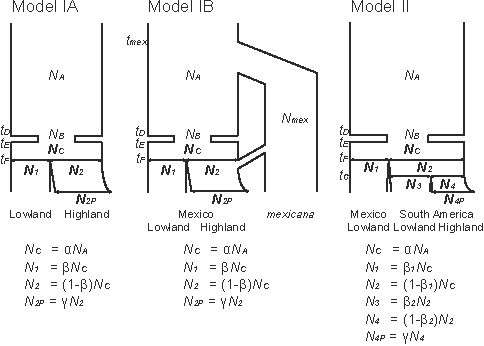
\includegraphics[width=0.5\textwidth]{fig/Fig3}
   \renewcommand{\baselinestretch}{0.9}
   \vspace{-3mm}
   \caption{ Demographic models of maize low- and highland populations.  Parameters in bold were estimated in this study.  See text for details.
   }
\vspace{-6mm}
    \label{model}
  \end{center}
\end{figure}
%%%%%%%%%%%%%%%%%%%%%%%%%%%%%%%%%%%%%%%%% FIGURE

\subsubsection{Model IA}
This model is applied to the Mexican and S. American populations.
We assume the ancestral diploid population representing \emph{parviglumis} follows a standard Wright-Fisher model with constant size.  
The size of the ancestral population is denoted by $N_A$.
At $t_D$ generations ago, the bottleneck event begins at domestication, and at $t_E$ generations ago, the bottleneck ends.  
The population size and duration of the bottleneck are denoted by $N_B$ and $t_B=t_D-t_E$, respectively.  
The population size recovers to $N_C=\alpha N_A$ in the lowlands.  
Then, the highland population is differentiated from the lowland population at $t_F$ generations ago.  
The size of the low- and highland populations at time $t_F$ is determined by a parameter $\beta$ such that the population is divided by $\beta N_C$ and $(1-\beta)N_C$.  
We assume that the population size in the lowlands is constant but that the highland population experiences exponential expansion after divergence: its current population size is $\gamma$ times larger than that at $t_F$. \\

%jri{isn't this really a shrinking population in the lowlands, since $\beta N_C<N_C$ ? wouldn't we want instead for lowlands to stay at $N_C$ and a new population branching off?  how much do we worry about this?}
%\st{actually, our conclusion holds when I assumed the pop size of lowlands stays at $N_C$.  However, the likelihood is a bit better in my original model.}

\subsubsection{Model IB}
We expand Model IA for the Mexican populations by incorporating admixture from the teosinte \emph{mexicana} to the highland Mexican maize population.  
The time of differentiation between \emph{parviglumis} and \emph{mexicana} occurs at $t_{mex}$ generations ago.  
The \emph{mexicana} population size is assumed to be constant at $N_{mex}$.  
At $t_F$ generations ago, the Mexican highland population is derived from admixture between the Mexican lowland population and a portion $P_{mex}$ from the teosinte \emph{mexicana}.\\  

\subsubsection{Model II}
The final model includes the Mexican lowland, S. American lowland and highland populations.  
This model was used for simulating SNPs with ascertainment bias (see below).  
At time $t_F$, the Mexican and S. American lowland populations are differentiated, and the sizes of populations after splitting are determined by $\beta_1$.  
At time $t_G$, the S. American lowland and highland populations are differentiated, and the sizes of populations at this time are determined by $\beta_2$.  
As in Model IA, the S. American highland population is assumed to experience population growth with the parameter $\gamma$.\\

Estimates of a number of our model parameters were available from previous work.    
$N_A$ was set to 150,000 using estimates of the composite parameter $4N_A\mu \sim 0.018$ from \emph{parviglumis}  \cite[]{Eyre-Walker_1998_9539756,Tenaillon_2001_11470895,Tenaillon_2004_15014173,Wright_2005_15919994,Ross-Ibarra_2009_19153259} and an estimate of the mutation rate $\mu \sim 3\times 10^{-8}$ \cite[]{Clark_2005_16079248} per site per generation.  
The severity of the domestication bottleneck is represented by $k=N_B/t_B$ \cite[]{Eyre-Walker_1998_9539756,Wright_2005_15919994}, and following \cite{Wright_2005_15919994} we assumed $k=2.45$ and $t_B=1,000$ generations.  
Taking into account archaeological evidence \cite[]{Piperno_2009_19307570}, we assume $t_D=9,000$ and $t_E=8,000$.  
We further assumed $t_F=6,000$ for Mexican populations in Models IA and IB \cite[]{Piperno_2006_69}, $t_F=4,000$ for S. American populations in Model IA \cite[]{Perry_2006_16511492,Grobman_2012_22307642}, and $t_{mex}=60,000$, $N_{mex}=160,000$ \cite[]{Ross-Ibarra_2009_19153259}, and $P_{mex}=0.2$ \cite[]{vanHeerwaarden_2011_21189301} for Model IB. 
For both Models IA and IB, we inferred three parameters ($\alpha$, $\beta$ and $\gamma$), and, for Model II, we fixed $t_F=6,000$ and $t_G=4,000$ \cite[]{Piperno_2006_69,Perry_2006_16511492,Grobman_2012_22307642}  and estimated the remaining four parameters ($\alpha$, $\beta_1$, $\beta_2$ and $\gamma$).

\subsection*{Population differentiation}
We used our inferred demographic model to generate a null distribution of $F_{ST}$.
As implemented in $\delta a \delta i$ \cite[]{Gutenkunst_2009_19851460}, we calculated an expected JFD given estimated demographic parameters and the sample sizes from our highland and lowland populations.
Then, we converted the JFD into the distribution of $F_{ST}$ values.
The \emph{P}-value of a SNP was calculated by $P(F_{ST\_E}\geq F_{ST\_O}|p\pm 0.05) = P(F_{ST\_E}\geq F_{ST\_O} \cap p\pm 0.05)/P(p\pm 0.05)$, 
where $F_{ST\_O}$ and $F_{ST\_E}$ are observed and expected $F_{ST}$ values and $p\pm 0.05$ is the set of loci with mean allele frequencies within 0.05 of the mean allele frequency of the SNP across both highland and lowland populations.

Generating the null distribution of differentiation for the MaizeSNP50 data requires accounting for ascertainment bias. 
Evaluation of genetic clustering in our data (not shown) coincides with previous work \cite[]{Hufford_2012_22660546} in suggesting that the two inbred lines most important in the ascertainment panel (B73 and Mo17) are most closely related to Mexican lowland maize.  
We thus added two additional individuals to the Mexican lowland population and generated our null distribution using only SNPs for which the two individuals had different alleles.
For model IA in S. America we added two individuals at time $t_F$ to the ancestral population of the S. American lowland and highland populations because the Mexican lowland population was not incorporated into this model. 
For each combination of sample sizes in lowland and highland populations, we generated a JFD from $10^7$  SNPs using the software {\sf ms} \cite[]{Hudson_2002_11847089}.
Then, we calculated \emph{P}-values from the JFD in the same way.
We calculated $F_{ST}$ values for all SNPs that had $\geq10$ individuals with no missing data in all four populations and showed no departure from HWE at the 0.5\% (GBS) or 5\% (MaizeSNP50) level. 

%\jri{we don't correct for allele frequency (or heterozygosity) in our Fst outlier analysis do we?  if not, this is a problem I think.}
%\st{I did.  No essential change}

%\jri{do we use all GBS data in the Fst outlier test, or just silent SNPs? we should be able to use nonsynonymous too, right?}
%\st{I used all.}

\subsection*{Haplotype sharing test}
We performed a \underline{p}airwise \underline{h}aplotype \underline{s}haring (PHS) test to detect further evidence of selection, following \cite{Toomajian_2006_16623598}.  
To conduct this test, we first imputed and phased the combined SNP data (both GBS and MaizeSNP50) using the {\sf fastPHASE} software version 1.4.0 \cite[]{Scheet_2006_16532393}.  
As a reference for phasing, we used data (excluding heterozygous SNPs) from an Americas-wide sample of 23 partially inbred landraces from the Hapmap v2 data set  \cite[]{Chia_2012_22660545}.  
We ran {\sf fastPHASE}  with default parameter settings.  
PHS was calculated for an allele \emph{A} at position $x$ by

\begin{equation}
  \label{phs-1}
  \begin{array}{l}
  \displaystyle{
PHS_{x_A} = \sum^{p-1}_{i=1}\sum^{p}_{j=i+1}Z_{ijx}  / \Bigl( \begin{array}{c} p \\ 2 \\ \end{array} \Bigr) 
- \sum^{n-1}_{i=1}\sum^{n}_{j=i+1}Z_{ijx}  / \Bigl( \begin{array}{c} n \\ 2 \\ \end{array} \Bigr) 
  }
  \end {array} 
  \textrm{,}
\end{equation}
\noindent where $n$ is the sample size of haploids, $p$  is the number of haploids carrying the allele $A$ at position $x$, and

\begin{equation}
  \label{phs-2}
  \begin{array}{l}
  \displaystyle{
Z_{ijx} = \frac{ d_{ijx} - \bar{d_{ij}} }{ \sigma_{ij} }
  }
  \end {array} 
  \textrm{,}
\end{equation}
\noindent where $d_{ijx}$ is the genetic distance over which individuals $i$ and $j$ are identical surrounding position $x$, $\bar{d_{ij}}$ is the genome-wide mean of distances over which individuals are identical, and $\sigma_{ij}$ is the standard deviation of the distribution of distances.  
The \emph{P}-value for each allele was calculated as the proportion of alleles of the same frequency genome-wide that have a larger PHS value. 

Genetic distances were obtained for the MaizeSNP50 data \cite[]{Ganal_2011_22174790} and fit using a tenth degree polynomial curve to all SNPs (data not shown).
 
%%%% PLR:
\subsection*{Theoretical evaluation of convergent evolution }
We build on results from \cite[]{ralph2014convergent} to assess whether the abundance and degree of coincidence of presumably adaptive high-$F_{ST}$ alleles is consistent with what is known about the population history of maize, we evaluated the rate at which we expect an allele that provides a selective advantage at higher elevation to arise by new mutation in a highland region ($\mutrate$), and the rate at which such an allele already present in the Mexican highlands would transit the intervening lowlands and fix in the Andean highlands ($\migrate$).
% We suggest below that many of the high-$F_{ST}$ alleles are locally adaptive, and the degree of coincidence between highland regions informs us about whether these adaptations occurred convergently, or if alleles were transmitted between the two by migration. 
We assume alleles adapted in the highlands are slightly deleterious at lower elevation, consistent with empirical findings in reciprocal transplant experiments in Mexico \cite[]{Mercer2008}.
These numbers depend most strongly on the population density, the selection coefficient, and the rate at which seed is transported long distances and replanted.
To obtain specific predictions, we computed $\mutrate$ and $\migrate$ at various parameter values.
We also checked these with simulations and more detailed computations, described in the Appendix.
Here we describe the mathematical details; readers may skip to the results without loss of continuity.\\

%To calculate the rate at which new mutations appear and fix in a highland population, $\mutrate$, we multiplied the total population size of the highlands by the mutation rate per generation.
\subsubsection{Demographic model}
Throughout, we followed \citet{vanHeerwaarden2010} in constructing a detailed demographic model for domesticated maize.
We assume fields of $N=10^5$ plants are replanted each year from $N_f=561$ ears, either from completely new stock (with probability $p_e=0.068$), from partially new stock (a proportion $r_m=0.2$ with probability $p_m=0.02$), or  otherwise entirely from the same field.
Each plant is seed parent to all kernels of its own ears, but can be pollen parent to kernels in many other ears; a proportion $m_g=0.0083$ of the pollen-parent kernels are in other fields.
Wild-type plants have an average of $\mu_E=3$ ears per plant, and ears have an average of $N/N_f$ kernels; each of these numbers are Poisson distributed.
The mean number of pollen-parent kernels, and the mean number of kernels per ear, is assumed to be $(1+s_b)$ times larger for individuals heterozygous for the selected allele.
Migration is mediated by seed exchange -- when fields are replanted, the seed is chosen from a random distance away with mean $\sigma_s=50$km, but plants only pollinate other plants belonging to the same village (distance 0).
Each individual can have offspring in three categories: local seed, local pollen, and migrant seed; the mean numbers of each of these are determined by the condition that the population is stable (i.e. wild-type, diploid individuals have on average 2 offspring) except that heterozygotes have on average $(1+s_b)$ offspring that carry the selected allele.
Each ear has a small chance of being chosen for replanting, so the number of ears replanted of a given individual is Poisson, and assuming that pollen is well-mixed, the number of pollen-parent kernels is Poisson as well.
Each of these numbers of offspring has a mean that depends on whether the field is replanted with new stock, and whether ears are chosen from this field to replant other fields, so the total number of offspring is actually a mixture of Poissons; these means, and more details of the computations, are found in Appendix \ref{apx:demographic_model}.
At these parameter values, we compute that the variance in number of offspring, $\xi^2$, is between 20 (for wild-type) and 30 (for $s_b=0.1$), and the dispersal distance (mean distance between parent and offspring) is $\sigma=1.8$km.\\

\subsubsection{New mutations}
The rate at which new mutations appear and fix in a highland population, which we denote $\mutrate$, is equal to the total population size of the highlands multiplied by the mutation rate per generation and by the chance that a single such mutation successfully fixes (i.e.\ is not lost to drift).
The probability that a single new mutant allele providing benefit $s_b$ to heterozygotes at high elevation will fix locally in the high elevation population is approximately $2s_b$ divided by the variance in offspring number \citep{jagers1975branching}.
The calculation above is not quite correct, as it neglects migration across the altitudinal gradient, but exact numerical calculation of the chance of fixation of a mutation as a function of the location where it first appears indicates that the approximation is quite good (see Figure~\ref{sfig:prob_estab}); for theoretical treatment see \citet{pollak1966survival} or \citet{barton1987establishment}.

 %\plr{could alternatively: (a) describe the math; or (b) cut this down further.}
 %I actually like this as is, but think we should expand math as separate appendix. my thinking is math will be of interest to a subset of audience, so perhaps best presented fully but at end. thoughts?
 %\plr{added a signpost for non-mathey readers to skip this at the start}

Concretely, the probability that a new mutation destined for fixation will arise in a patch of high-elevation habitat of area $A$ in a given generation is a function of the density of maize per unit area $\rho$, the selective benefit $s_b$ it provides, the mutation rate $\mu$, and the variance in offspring number $\xi^2$.
In terms of these parameters, the rate of appearance is 
\begin{align} \label{eqn:mutrate}
  \mutrate = \frac{2 \mu \rho A s_b}{\xi^2} .
\end{align}

\subsubsection{Migration}
A corresponding expression for the chance that an allele moves from one highland population to another is harder to intuit, and is addressed in more depth in \citep{ralph2014convergent}.
If an allele is beneficial at high elevation and fixed in the Mexican highlands but is deleterious at low elevations, then at equilibrium it will be present at low frequency at migration-selection balance \citep{slatkin1973geneflow} in nearby lowland populations.
This equilibrium frequency decays exponentially with distance, so that the highland allele is present at distance $R$ from the highlands at frequency $C \exp(- R \sqrt{2s_m} / \sigma)$, where $s_m$ is the deleterious selection coefficient for the allele in low elevation, $\sigma$ is the mean dispersal distance, and $C$ is a constant depending on geography ($C\approx 1/2$ is close).
Multiplying this frequency by a population size gets the predicted number (average density across a large number of generations) of individuals carrying the allele.
Therefore, in a lowland population of size $N$ at distance $R$ from the highlands, $(N/2)  \exp(- R \sqrt{2s_m} / \sigma)$ is equal to the probability that there are any highland alleles present, multiplied by the expected number of these given that some are present.
Since the latter is at least 1, this puts an upper bound on the rate of migration
%the chance there are any present in a given generation is no more than $(N/2) \exp(- R \sqrt{2s_m} / \sigma)$, and so this puts an upper bound on $\migrate$.
%Therefore, we would need to wait $\Tmig = (2/N)\exp(R \sqrt{2s_m} / \sigma)$ generations for a rare such excursion to occur.
%In other words, we can bound the rate of migration by
\begin{align}
  \migrate \le (N/2)  \exp(- R \sqrt{2s_m} / \sigma),
\end{align}
and we we would need to wait $\Tmig = 1/\migrate$ generations for a rare such excursion to occur.
%with $N$ being the total size of the unadapted highland population, and $R$ the distance from the adapted to the yet-unadapted highland populations.
This calculation omits the probability that such an allele fixes ($\approx 2s_b/\xi^2$), but since such alleles arrive by migration, this omission is unlikely a large effect and is conservative.








\section*{Results}

%%%%%%%%%%%%%%%%%%%%%%%%%%%%%%%%%%%%%%%%%%%%%%%%%%%%%%%%%%%%
\renewcommand{\arraystretch}{1.1}
\begin{table}[tb]

\begin{center}
 \caption[]{$F_{ST}$ of synonymous and noncoding GBS SNPs}
  \textbf{}\\[-2mm]
{\fontsize{7}{9}\sf
    \begin{tabular}{llccccccl}
    \hline
    & & \\[-3mm]
	&		&	\multicolumn{2}{c}{Mexico}		&	\multicolumn{2}{c}{S. America}		\\
	&		&	Lowlands	&	Highlands	&	Lowlands	&	Highlands	\\
      \hline
    & & \\[-3mm]
Mexico	&	Lowlands	&	--		&			&			&		\\
		&	Highlands	&	0.0244	&	--		&			&		\\
S. America		&	Lowlands	&	0.0227	&	0.0343	&	--		&		\\
		&	Highlands	&	0.0466	&	0.0534	&	0.0442	&	--	\\ [1mm]
    \hline
    \end{tabular}
    \label{FstP}  % caption is needed to make this work
}
\end{center}
\end{table}
\renewcommand{\arraystretch}{1}
%%%%%%%%%%%%%%%%%%%%%%%%%%%%%%%%%%%%%%%%%%%%%%%%%%%%%%%%%%%%

 %%%%%%%%%%%%%%%%%%%%%%%%%%%%%%%%%%%%%%%%%%%%%%%%%%%%%%%%%%%%
\renewcommand{\arraystretch}{1.1}
\begin{table}[tb]

\begin{center}
 \caption[]{Estimated parameters of population size model}
  \textbf{}\\[-2mm]
{\fontsize{7}{11}\sf
    \begin{tabular}{lcccccccl} \hline
       & & \\[-3mm]
     Mexico  & \multicolumn{2}{c}{Model IA}  &\multicolumn{2}{c}{Model IB}\\[0.1cm]
    \hline
    & & \\[-3mm]
   & Likelihood   & $-$5592.80 & Likelihood       &  $-$4654.79 \\
   &$\alpha$      & 0.92             & $\alpha$        & 1.5 \\
   &$\beta$        & 0.38             & $\beta$          & 0.76\\ 
   &$\gamma$   & 1                   &  $\gamma$   & 1\\ 
      \hline
    & & \\[-3mm]
    S. America  & \multicolumn{2}{c}{Model IA}  &\multicolumn{2}{c}{Model II}\\[0.1cm]
        \hline
     & & \\[-3mm]
      & Likelihood   &  $-$3855.28 & Likelihood     &  $-$8044.71 \\
      &$\alpha$      & 0.52              & $\alpha$       & 1.0 \\
      &$\beta$        & 0.97             & $\beta_1$      & 0.64\\ 
      &$\gamma$   & 88                &  $\beta_2$     & 0.95\\ 
      &                    &                     &  $\gamma$    & 54\\ [1mm]
    \hline
%    \multicolumn{9}{l}{$^{a}$ The groups were based on phylogenetic analysis in fig.~\ref{tree}\emph{A}}\\
    \end{tabular}
    \label{param}  % caption is needed to make this work
}
\end{center}
\end{table}
\renewcommand{\arraystretch}{1}
%%%%%%%%%%%%%%%%%%%%%%%%%%%%%%%%%%%%%%%%%%%%%%%%%%%%%%%%%%%%


\subsection*{Samples and data}

We sampled 94 maize landraces from four distinct regions in the Americas (Table \ref{srkid}): the lowlands of Mexico/Guatemala ($n=24$) and northern South America ($n=23$) and the highlands of the Mexican Central Plateau ($n=24$) and the Andes ($n=23$). 
Samples were genotyped using the MaizeSNP50 Beadchip platform (``MaizeSNP50''; $n=94$) and genotyping-by-sequencing (``GBS''; $n=87$). 
After filtering for Hardy-Weinberg genotype frequencies and minimum sample size $\geq10$ in each of the four populations (see Materials and Methods) 91,779 SNPs remained, including 67,828 and 23,951 SNPs from GBS and MaizeSNP50 respectively.  

\subsection*{Population structure}

We performed a {\sf STRUCTURE} analysis \cite[]{Pritchard_2000_10835412,Falush_2003_12930761} of our landrace samples, varying the number of groups from $K$ = 2 to 6 (Figure~\ref{map}, Figure~\ref{supp:struct}). 
Most landraces were assigned to groups consistent with \emph{a priori} population definitions, but admixture between highland and lowland populations was evident at intermediate elevations ($\sim1700$m).  Consistent with previously described scenarios for maize diffusion \cite[]{Piperno_2006_69}, we find evidence of shared ancestry between lowland Mexican maize and both Mexican highland and S. American lowland populations.  Pairwise $F_{ST}$ among populations reveals low overall differentiation (Table \ref{FstP}), and the higher $F_{ST}$ values observed in S. America are consistent with the decreased admixture seen in {\sf STRUCTURE}.  Archaeological evidence supports a more recent colonization of the highlands in S. America  \cite[]{Piperno_2006_69,Perry_2006_16511492,Grobman_2012_22307642}, suggesting that the observed differentiation may be the result of a stronger bottleneck during colonization of the S. American highlands.  

%%%%%%%%%%%%%%%%%%%%%%%%%%%%%%%%%%%%%%%%%% FIGURE
\begin{figure}[tb]   
  \begin{center}
   \vspace{-0mm}
   %\includegraphics[width=0.23\textwidth]{figs/model}
   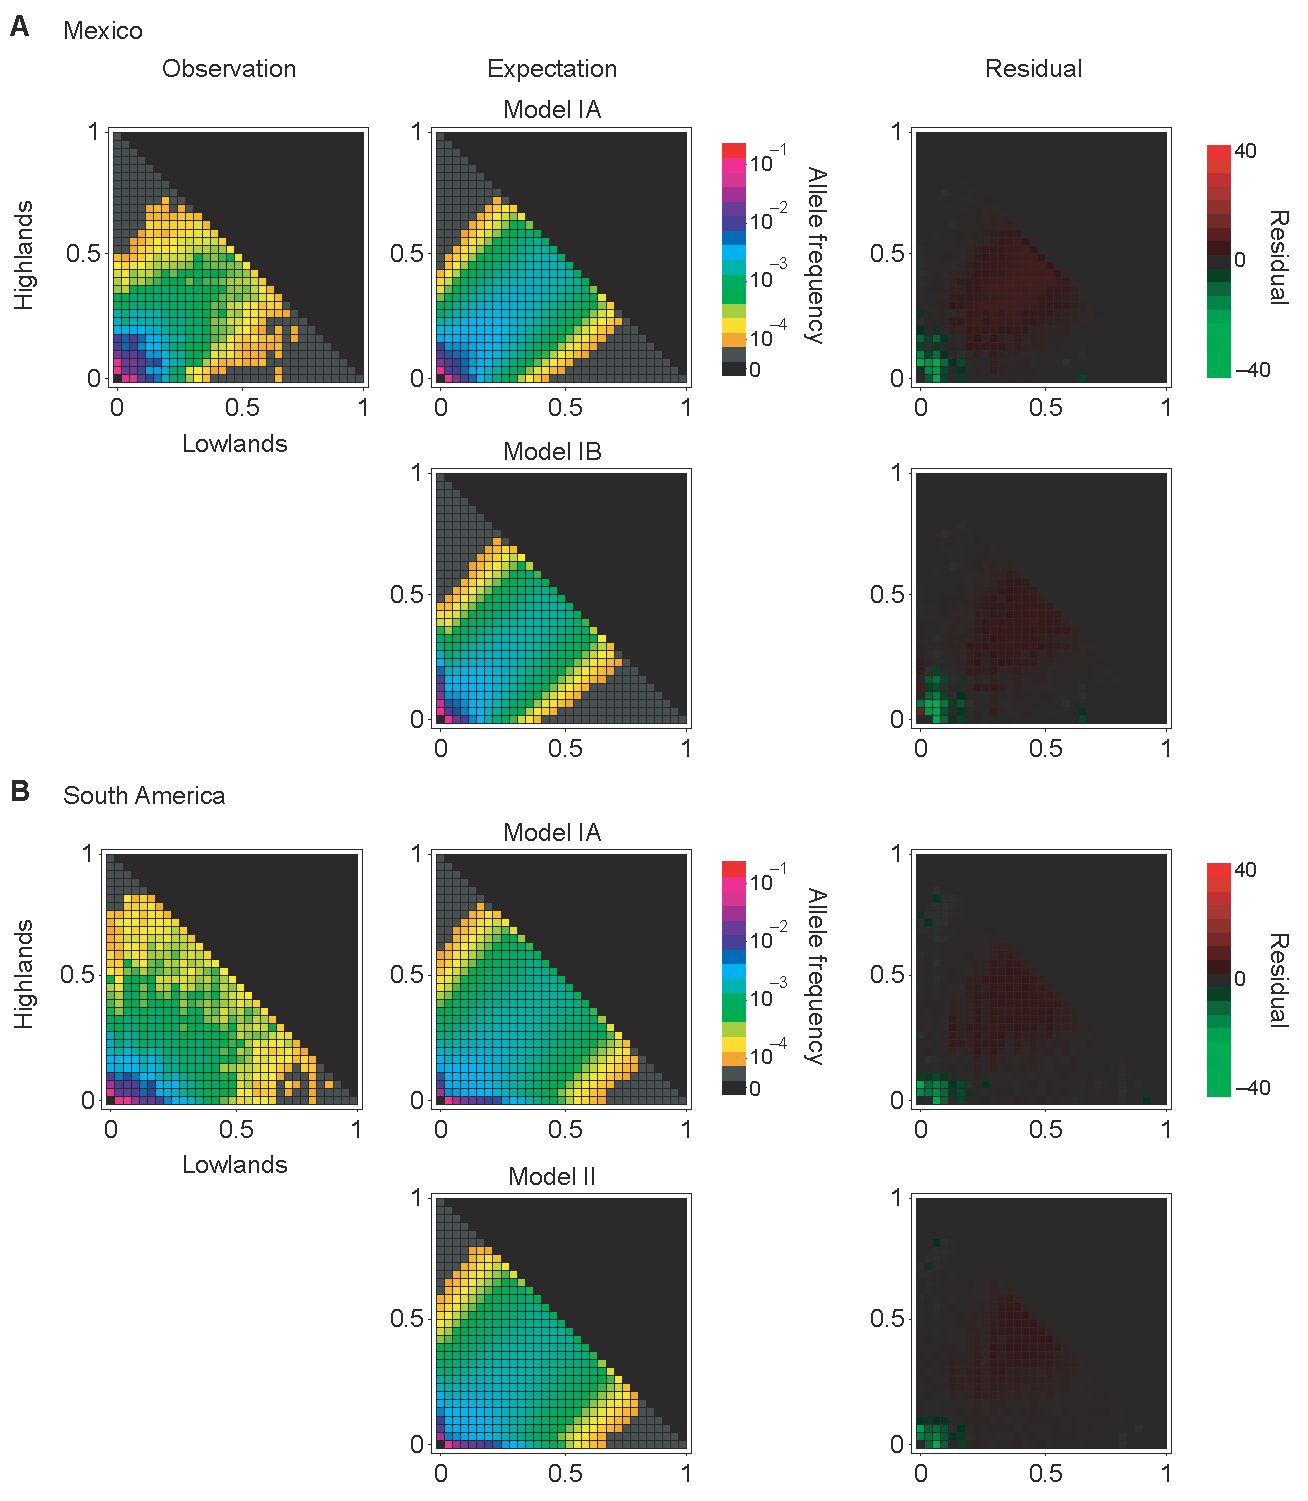
\includegraphics[width=0.5\textwidth]{fig/Fig4}
   \renewcommand{\baselinestretch}{0.9}
   \vspace{-3mm}
   \caption{Observed and expected joint distributions of minor allele frequencies in lowland and highland populations in (A) Mexico and (B) S. America. Residuals are calculated as  $(\mbox{model}-\mbox{data})/\sqrt[]{\mbox{model}}$}
\vspace{-6mm}
    \label{JFD}
  \end{center}
\end{figure}
%%%%%%%%%%%%%%%%%%%%%%%%%%%%%%%%%%%%%%%%%% FIGURE

\subsection*{Population differentiation}

To provide a null expectation for allele frequency differentiation, we used the joint site frequency distribution (JFD) of lowland and highland populations to estimate parameters of two demographic models  using the maximum likelihood method implemented in $\delta a \delta i$ \cite[]{Gutenkunst_2009_19851460}.  
All models incorporate a domestication bottleneck \cite[]{Wright_2005_15919994} and population differentiation between lowland and highland populations, but differ in their consideration of admixture and ascertainment bias (Figure~\ref{model}; see Materials and Methods for details).

Estimated parameter values are listed in Table~\ref{param}; while the observed and expected JFDs were quite similar for both models,  residuals indicated an excess of rare variants in the observed JFDs in all cases (Figure~\ref{JFD}). 
Under both models IA and IB,  we found expansion in the highland population in Mexico to be unlikely, but a strong bottleneck followed by population expansion is supported in S. American maize in both models IA and II.  
The likelihood value of model IB was higher than the likelihood of model IA by 850 units of log-likelihood (Table~\ref{param}), consistent with analyses suggesting that introgression from \textit{mexicana} played a significant role during the spread of maize into the Mexican highlands \cite[]{Profford_2013}. 

In addition to the parameters listed in Figure~\ref{model}, we investigated the impact of varying the domestication bottleneck size ($N_B$).  
Surprisingly, $N_B$ was estimated to be equal to $N_C$, the population size at the end of the bottleneck, and the likelihood of $N_B<N_C$ was much smaller than for alternative parameterizations (Table~\ref{param},~\ref{supp:param}). 

Comparisons of our empirical $F_{ST}$ values to the null expectation simulated under our demographic models allowed us to identify significantly differentiated SNPs between lowland and highland populations. In all cases, observed $F_{ST}$ values were quite similar to those generated under our null models (Figure~\ref{FstDist}), and model choice -- including the parameterization of the domestication bottleneck -- had little impact on the distribution of estimated \emph{P}-values (Figure~\ref{fig:qq}). 
We show results under Model IB for Mexican populations and Model II for S. American populations.
We chose $P<0.01$ as an arbitrary cut-off for significant differentiation between lowland and highland populations, and identified 687 SNPs in Mexico (687/76,989=0.89\%) and 409 SNPs in South America (409/63,160=0.65\%) as outliers (Figure~\ref{PvDist}). Different cutoff values (0.05, 0.001) gave qualitatively identical results (data not shown).
SNPs with significant $F_{ST}$ $P$-values were enriched in intergenic regions rather than protein coding regions (60.0\% vs. 47.9\%, Fisher's Exact Test $P < 10^{-7}$ for Mexico; 62.0\% vs. 47.8\%, FET $P<10^{-5}$ for S. America). 

%%%%%%%%%%%%%%%%%%%%%%%%%%%%%%%%%%%%%%%%%% FIGURE
\begin{figure}[tb]   
  \begin{center}
   \vspace{-0mm}
   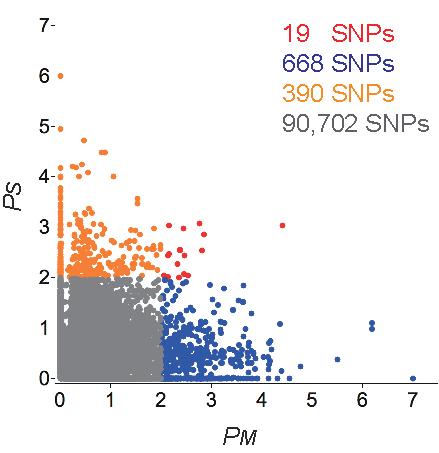
\includegraphics[width=0.4\textwidth]{fig/Fig6}
   \renewcommand{\baselinestretch}{0.9}
   \vspace{-3mm}
   \caption{Scatter plot of $-\log_{10} P$-values of observed $F_{ST}$ values based on simulation from estimated demographic models. $P$-values are shown for each SNP in both Mexico (Model IB; $P_M$ on $x$-axis) and S. America (Model II; $P_S$ on $y$-axis).  
   Red, blue, orange and gray dots represents SNPs showing significance in both Mexico and S. America, only in Mexico, only in S. America, respectively (see text for details).
   The number of SNPs in each category is shown in the same color as the points.} 
\vspace{-6mm}
    \label{PvDist}
  \end{center}
\end{figure}
%%%%%%%%%%%%%%%%%%%%%%%%%%%%%%%%%%%%%%%%%% FIGURE

\subsection*{Patterns of adaptation}

Given the historical spread of maize from an origin in the lowlands, it is tempting to assume that the observation of significant population differentiation at a SNP should be primarily due to an increase in frequency of adaptive alleles in the highlands.
To test this hypothesis, we sought to identify the adaptive allele at each locus using comparisons between Mexico and S. America as well as to \emph{parviglumis} (See Supplementary Text  for details).  
Consistent with predictions, we infer that differentiation at 72.3\% (264) and 76.7\% (230) of SNPs in Mexico and S. America is due to adaptation in the highlands after excluding  SNPs with ambiguous patterns likely due to recombination. 
The majority of these SNPs show patterns of haplotype variation (by the PHS test) consistent with our inference of selection (Supplementary Text and Table~\ref{supp:phs}).
   
Convergent evolution at the nucleotide level should be reflected in an excess of SNPs showing significant differentiation between lowland and highland populations in both Mexico and S. America. 
Although the 19 SNPs showing $F_{ST}$ \emph{P}-values  $<0.01$ in both Mexico ($P_M$) and S. America ($P_S$) is statistically greater than the $\approx 5$ expected ($48,370\times 0.01 \times 0.01 \approx 4.8$; $\chi^2$-test, $P\ll0.001$), it nonetheless represents a small fraction ($\approx 7-8\%$) of all SNPs showing evidence of selection.
This paucity of shared selected SNPs does not appear to be due to our demographic model: a model-free approach based on the top 1\% highest $F_{ST}$ values finds no shared adaptive SNPs between Mexican and S. American highland populations. 
For 13 of 19 SNPs showing putative evidence of shared selection we could use data from \textit{parviglumis} to infer whether these SNPs were likely selected in lowland or highland conditions (Supplemental Text).  
Surprisingly, SNPs identified as shared adaptive variants more frequently showed segregation patterns consistent with lowland  (10 SNPs) rather than highland adaptation (2 SNPs). %(1 SNP with an ambiguous pattern). 

We also investigated how often different SNPs in the same gene may have been targeted by selection. 
To search for this pattern, we considered all SNPs within 10kb of a transcript as part of the same gene, though SNPs in an miRNA or second transcript within 10kb of the transcript of interest were excluded.  
We classified SNPs showing significant $F_{ST}$ in Mexico, S. America or in both regions into 778 genes. 
Of these, 485 and 277 genes showed Mexico-specific and SA-specific significant SNPs, while 14 genes contained at least one SNP with a pattern of differentiation suggesting convergent evolution and 2 genes contained both Mexico-specific and SA-specific significant SNPs. 
Overall, however, fewer genes showed evidence of convergent evolution than expected by chance (permutation test; $P<10^{-5}$). 
Despite similar phenotypes and environments, we thus see little evidence for convergent evolution at either the SNP or the gene level.  

\subsection*{Comparison to theory}

% # \mutrate computation:
% A <- 500; rho <- 5000; sb <- 10^(-(1:4)); xisq <- 30
% sapply( 10^c(-5,-8), function (mu) mu * (2 * rho * A * sb)/xisq )

Given the limited empirical evidence for convergent evolution at the molecular level, we took advantage of recent theoretical efforts \cite[]{ralph2014convergent} to assess the degree of convergence expected under a spatially explicit population genetic model (see Materials and Methods).
Our modeling estimates assume a maize population density $\rho$ of the highlands to be around (0.5 ha field/person) $\times$ (0.5 people/km$^2$) $\times$ ($2\times 10^4$ plants per ha field) $=$ 5,000 plants per km$^2$.
The area of the Andean highlands is around $A=500\text{km}^2$, leading to a total population of $A \rho = 2.5 \times 10^6$. 
Assuming an offspring variance of $\xi^2 = 30$, we can then compute the waiting time $\Tmut=1/\mutrate$ for a new beneficial mutation to appear and fix.
We observe that even if there is relatively strong selection for an allele at high elevation ($s_b=0.01$), a single-base mutation with mutation rate $\mu=10^{-8}$ would take at least 60,000 generations to appear and fix.
Because $\Tmut$ scales approximately linearly with both the selection coefficient and the mutation rate, strong selection and the existence of multiple equivalent mutable sites could reduce this time. 
For example, if any one of 10 sites within a gene could have equivalent strong selective benefit ($s_b=0.1$), $\Tmut$ would be reduced to 600 generations. \jri{Peter please check this paragraph to make sure numbers and text look OK.}

% # Tmig computation:
% A <- 500; rho <- 5000; sm <- 10^(-(1:4)); xisq <- 30; sigma <- 1.8
% 1/(sqrt(2*sm)/sigma)
% sapply( 1000*(1:4), function (R) 1 / ( A * rho * ( sqrt(2*sm) / xisq ) * exp(- sqrt(2*sm)*R/sigma ) ) )
% Ne <- (561/10^5)*A*rho 
% Ne  # = 14025
% sapply( 1000*(1:4), function (R) 1 / ( Ne * exp(- sqrt(2*sm)*R/sigma ) ) )

Gene flow between highland regions could also generate patterns of shared adaptive SNPs.
From our demographic model we have estimated a mean dispersal distance of $\sigma \approx 1.8$ kilometers per generation.
With selection against the highland allele in low elevations $10^{-1} \ge s_m \ge 10^{-4}$, the distance $\sigma/\sqrt{2s_m}$ over which the frequency of a highland-adaptive, lowland-deleterious allele decays into the lowlands is still short: between 4 and 150 kilometers.
Since the Mexican and Andean highlands are around 4,000 km apart, the time needed for a rare allele with weak selective cost $s_m=10^{-4}$ in the lowlands to transit between the two highland regions is $\Tmig \approx 4 \times 10^{10}$ generations. 
However, shorter distances could be transited more quickly -- if the distance between highland patches $R$ is 1,000 km (or if $\sigma$ is four times larger) then the same allele would be expected to transit between populations in approximately 2 generations.
The waiting time $\Tmig$ is  strongly dependent on the magnitude of the deleterious selection coefficient, however: with $s_m=10^{-3}$, for example $\Tmig$ is $1.6 \times 10^7$ generations over 1,000km.
%Since the Mexican and Andean highlands are around 4,000 km apart, the time needed for a rare allele with selective cost $s_m=10^{-3}$ in the lowlands to transit between the two highland regions is $\Tmig \approx 5 \times 10^{34}$ generations. 
%The waiting time $\Tmig$, however,is is strongly dependent on the magnitude of the deleterious selection coefficient: for example, with $s_m=10^{-3}$, $\Tmig$ is $2.3 \times 10^6$ generations.
\jri{Peter please check $\Tmig$ here is correct. Original sentence (see .tex) didn't give numbers for waiting time that jived with what I get from R code in .tex}

Finally, a coalescent approach allows us to also estimate the distance travelled for a beneficial highland alleles which is neutral in lowland environments.  After $m=1,000$ generations, there are approximately $n=1,000$ lineages remaining and of these the furthest has travelled  $\sqrt{2 \sigma^2 m \log n} \approx 212$km from the highlands.  The distance travelled, however, does not scale linearly with time, such that at  $m=6000$ generations the furthest alleles is $\approx 518$km from its highland origin. \jri{Peter I'm confused here. If the above is correct it argues a neutral allele will travel a \emph{shorter} distance than a deleterious allele? 1000km would take neutral allele >6K generations but in the previous paragraph a deleterious allele with $s_m=10^{-4}$ does it in 2 generations.}

%With $n=1000$, the typical distance to the furthest displacement after $m=1000$ generations is $\sqrt{2 \sigma^2 m \log n} \approx 212$km; after $m=6000$ generations it is $\approx 518$km.
%In either case, the chance that the maximum is larger than 1,000km after 6,000 generations is well less than $10^{-4}$.
%Of course, this is under an equilibrium population model; and maize reached the Andean highlands only around 4,000 years ago.
%Nonetheless, this suggests that even highland-adapted alleles that are merely neutral in the lowlands would have difficulty moving between the Mexican and Andean highlands in a few thousand generations.

\subsection*{Alternative routes of adaptation}
The lack of both empirical and theoretical support for convergent adaptation at SNPs or genes led us to investigate alternative patterns of adaptation. 

We first sought to understand whether SNPs showing high differentiation between the lowlands and the highlands arose primarily via new mutations or were selected from standing genetic variation.  
We found that putatively adaptive variants in both Mexico and South America tended to segregate in the lowland population more often than other SNPs of similar mean allele frequency (85.3\% vs. 74.8\% in Mexico, FET {$P < 10^{-9}$ and 94.8\% vs 87.4\% in South America,  $P< 10^{-4}$).  
We extended this analysis by retrieving SNP data from 14 \emph{parviglumis} inbred lines included in the Hapmap v2 data set, using only SNPs with $n\geq10$ \cite[]{Chia_2012_22660545,Hufford_2012_22660546}.  
Again we found that putatively adaptive variants were more likely to be polymorphic in \emph{parviglumis} (78.3\% vs. 72.2\% in Mexico, FET {$P < 0.01$ and 80.2\% vs 72.8\% in South America,  $P< 0.01$).  

While maize in highland Mexico grows in sympatry with the highland teosinte \textit{mexicana}, maize in South America is outside the range of wild \textit{Zea} species, leading to a marked difference in the potential for adaptive introgression from wild relatives.
\citet{Pyhajarvi2013} recently investigated local adaptation in \textit{parviglumis} and \textit{mexicana} populations, characterizing differentiation between these subspecies using an outlier approach.
Genome-wide, only a small proportion of ($\sim 2-7\%$) of our putatively adaptive SNPs were identified by \citet{Pyhajarvi2013}, though these numbers are still in excess of expectations (FET $P<10^{-3}$ for S. America and $P<10^{-8}$ for Mexico; Table~\ref{tanja}).
The proportion of putatively adaptive SNPs shared with teosinte was twice as high in Mexico, however, leading us to evaluate our results in light of introgression identified by \citet{Profford_2013} from \textit{mexicana} into maize in the Mexican highlands.  

The proportion of putatively adaptive SNPs in introgressed regions of the genome in highland maize in Mexico was nearly four times higher than found in S. America (FET $P<10^{-11}$), while differences outside introgressed regions were much smaller (7.5\% vs. 6.2\%; Table \ref{supp:introgressed}). 
Furthermore, of the 77 regions identified as introgressed in \cite[]{Profford_2013}, more than twice as many contain at least one $F_{ST}$ outlier in Mexico as in S. America (23 compared to 9, one-tailed Z-test $P=0.0027$).
Excluding  putatively adaptive SNPs, mean $F_{ST}$ between Mexico and S. America is only slightly higher in introgressed regions (0.032) than across the rest of the genome (0.020), suggesting the enrichment of high $F_{ST}$ SNPs seen in Mexico is not simply due to neutral introgression of a divergent teosinte haplotype.  
\ref{supp:introgressed}


%When focusing on GUs, we identified 99/586 (14.5\%) and 22/466 (4.7\%) GUs of Mexico- and SA-specific significance in introgressed regions (Fisher's exact test, $P<10^{-6}$). 


    


\section*{Conclusions} \jri{ WE NEED A CONCLUSION! }
1. We successfully inferred demography and detected the candidates of adaptive loci to highland climates in Mexico and South America by utilizing GBS and 55-k chip.

2. The main conclusion is parallel adaptation is rare in maize highland adaptation.


\begin{acknowledgments}
  We appreciate the helpful comments of P. Morrell and the members of Ross-Ibarra lab and Coop labs.   
\jri{add in formal acknowledgement of USDA. use grant number from Joost's 2012 PNAS paper. also need to ask Ed for grant number for GBS data. }
\end{acknowledgments}

\bibliography{MZpara1,MZpara2,plr-hilo}
\bibliographystyle{geneticsT2}

\suppl

%%%%%%%
% put supplemental figures and tables here:
% e.g.
% \begin{figure}
% ...


%%%%%
% appendices to follow

\renewcommand{\thefigure}{A\arabic{figure}}
\renewcommand{\thetable}{A\arabic{table}}

\section*{Appendix}

\section{Details of the demographic model}
\label{apx:demographic_model}

Throughout we use in many ways the {\em branching process approximation} --
if an allele is locally rare, then for at least a few generations,
the fates of each offspring are nearly independent.
So, if the allele is locally deleterious, the total numbers of that allele behave as a subcritical branching process,
destined for ultimate extinction.
On the other hand, if the allele is advantageous,
it will either die out or become locally common, with its fate determined in the first few generations.
If the number of offspring of an individual with this allele is the random variable $X$, 
with mean $\E[X] = 1+s$ (selective advantage $s>0$), variance $\var[X]=\xi^2$, and $\P\{X=0\}>0$ (some chance of leaving no offspring),
then the probability of local nonextinction $p_*$ is approximately $p_* \approx 2s/\xi^2$ to a second order in $s$.
The precise value can be found by defining the generating function $\Phi(u) = \E[u^X]$; 
the probability of local nonextinction $p_*$ is the minimal solution to $\Phi(1-u) = 1-u$.
(This can be seen because: $1-p_*$ is the probability that an individual's family dies out;
this is equal to the probability that the families of all that individuals' children die out;
since each child's family behaves independently, if the individual has $x$ offspring, this is equal to $(1-p_*)^x$;
and $\Phi(1-p_*) = \E[(1-p_*)^X]$.)

If the selective advantage ($s$) depends on geographic location, 
a similar fact holds: index spatial location by $i \in 1, \ldots, n$,
and for $u = (u_1,u_2,\ldots,u_n)$ define the functions $\Phi_i(u) = \E[ \prod_j u_j^{X_{ij}} ]$,
where $X_{ij}$ is the (random) number of offspring that an individual at $i$ produces at location $j$.
Then $p_* = (p_{*1}, \ldots, p_{*n})$, the vector of probabilities that a new mutation at each location eventually fixes,
is the minimal solution to $\Phi(1-p_*) = 1-p_*$,
i.e.\ $\Phi_i(1-p_*) = 1-p_{*i}$.

%%%%% in rcode/maize_calcs.R
% # maize
% N <- 103359  # plants per field
% Nf <- 561    # ears to make next generation
% e <- 0.068   # prob of total seed stock replacement
% mg <- .0083  # pollen migration
% pm <- .02    # prob of partial stock addition
% m <- 0.2     # proportion of stock replaced
% eqvals <- c(1, iterroot( function (p) { 
%             p.dead <- e + (1/2)*(1-e)*(1-Nf/N)
%             return( p.dead * 1 + 
%                     (1/2)*(1-e)*exp(((1+sb)/p.dead)*( p - 1 )) + 
%                     ((1/2)*(1-e)*Nf/N)*exp(((N/Nf)*(1+sb)/(1-e))*( p - 1 )) 
%                 )
%         } ) )
% genfn <- function (f,selx,migr=.5) { 
%         (e + (1/2)*(1-e)*(1-Nf/N))* 1 + #  no offspring
%         (1/2)*(1-e)*exp(((1+selx)/(1-e))*( f + migr*diff(c(eqvals[1],f,eqvals[2]),differences=2) - 1 )) + # pollen, Poisson mean 1+s(x)
%         (1/2)*(1-e)*(Nf/N)*exp(((N/Nf)*(1+selx/(1-e)))*( f + migr*diff(c(eqvals[1],f,eqvals[2]),differences=2) - 1 )) # seed, Poisson mean (1+s(x))*N/Nf
%     }

Here we consider a linear habitat, so that the selection coefficient at location $\ell_i$ is $s_i = \min( s_b, \max( - s_d, \alpha \ell_i ) )$.
There does not seem to be a nice analytic expression for $p_*$ in this case,
but since $1-p_*$ is a fixed point of $\Phi$, the solution can be found by iteration:
$1-p_* = \lim_{n \to \infty} \Phi^n(u)$ for an appropriate starting point $u$.

\subsection{Maize model}

The migration and reproduction dynamics we use are taken largely from \citet{vanHeerwaarden2010}.  
On a large scale,
fields of $N$ plants are replanted each year from $N_f$ ears,
either from completely new stock (with probability $p_e$),
from partially new stock (a proportion $r_m$ with probability $p_m$),
or entirely from the same field.
Plants have an average of $\mu_E$ ears per plant, and ears have an average of $N/N_f$ kernels; \jri{what happens if we change mean ears per plant from 3 to 1?}
so a plant has on average $\mu_E N/N_f$ kernels, and a field has on average $\mu_E N$ ears and $\mu_E N^2/N_f$ kernels.
We suppose that a plant with the selected allele is pollen parent to $(1+s) \mu_E N/N_f$ kernels,
and also seed parent to $(1+s)\mu_E N/N_f$ kernels, still in $\mu_E$ ears.
The number of offspring a plant has depends on how many of its offspring kernels get replanted.
Some proportion $m_g$ of the pollen-parent kernels are in other fields, and may be replanted;
but with probability $p_e$ no other kernels (i.e.~those in the same field) are replanted.
Otherwise, with probability $1-p_m$ the farmer chooses $N_f$ of the ears from this field to replant
(or, $(1-r_m) N_f$ of them, with probability $p_m$);
this results in a mean number $N_f/N$ (or, $(1-r_m)N_f/N$) of the plant's ears of seed children being chosen,
and a mean number $1+s$ of the plant's pollen children kernels being chosen.
Furthermore, the field is used to completely (or partially) replant another's field with chance $p_e/(1-p_e)$ (or $p_m$);
resulting in another $N_f/N$ (or $r_m N_f/N$) ears and $1+s$ (or $r_m (1+s)$) pollen children being replanted elsewhere.
Here we have assumed that pollen is well-mixed within a field,
and that the selected allele is locally rare.
Finally, we must divide all these offspring numbers by 2,
since we look at the offspring carrying a particular haplotype, not of the diploid plant's genome.

The above gives mean values; to get a probability model we assume that every count is Poisson.
In other words, we suppose that the number of pollen children is Poisson with random mean $\lambda_P$,
and the number of seed children is a mixture of $K$ independent Poissons with mean $(1+s)N/N_f$ each,
where $K$ is the random number of ears chosen to replant, which is itself Poisson with mean $\mu_K$.
By Poisson additivity, the numbers of local and migrant offspring are Poisson,
with means $\lambda_P = \lambda_{PL} + \lambda_{PM}$ and $\mu_K = \mu_{KL} + \mu_{KM}$ respectively.
With probability $p_e$, $\lambda_{PM} = m_g(1+s)$ and $\mu_K = \lambda_{PL} = 0$.
Otherwise, with probability $(1-p_e)(1-p_m)$, $\mu_{KL} = N_f/N$ and $\lambda_{PL} = (1+s)(1-m_g)$;
and with probability $(1-p_e)p_m$, $\mu_{KL} = (1-r_m) N_f/N$ and $\lambda_{PL} = (1-r_m)(1+s)(1-m_g)$.
The migrant means are,
with probability $(1-p_e) p_e/(1-p_e) = p_e$, $\mu_{KM} = N_f/N$ and $\lambda_{PM} = 1+s$;
while with probability $(1-p_e) p_m$, $\mu_{KM} = r_m N_f/N$ and $\lambda_{PM} = (1+s)(r_m(1-m_g) + m_g)$,
and otherwise $\mu_{KM} = 0$ and $\lambda_{PM} = m_g(1+s)$.


\begin{table}[htb!!]
  \begin{center}
  \begin{tabular}{|cll|}
    \hline
    complete seed stock replacement prob & $p_e$     & 0.068 \\
    pollen migration rate                & $m_g$      & 0.0083 \\
    number of plants per field           & $N$        & $10^5$ \\
    number of ears used to replant       & $N_f$      & 561 \\
    mean ears per plant                  & $\mu_E$    & 3 \\
    partial stock replacement prob       & $p_m$      & 0.02 \\
    mean proportion stock replaced       & $r_m$      & 0.2 \\
    pollen migration distance            & $\sigma_p$ & 0 km \\
    seed replacement distance            & $\sigma_s$ & 50 km \\
    distance between demes               & $a$        & 15 km \\
    width of altitudinal cline           & $w$        & 62km \\
    deleterious selection coefficient    & $s_d$      & varies \\
    beneficial selection coefficient     & $s_b$      & varies \\
    slope of selection gradient          & $\alpha$   & $(s_d+s_b)/w$ \\
    variance in offspring number         & $\xi^2$    & varies \\
    maize population density             & $\rho$     & $5 \times 10^3$ \\
    area of highland habitat             & $A$        & 500 km$^2$ \\
    mean dispersal distance              & $\sigma$   & 1.8 km \\
    \hline 
  \end{tabular}
\end{center}
  \caption{Parameter estimates used in calculations, and other notation.
  \label{tab:parameters}
  }
\end{table}


\subsection{Math}

The generating function of a Poisson with mean $\lambda$ is $\phi(u;\lambda)=\exp(\lambda(u-1))$,
and the generating function of a Poisson($\mu$) sum of Poisson($\lambda$) values is $\phi(\phi(u;\lambda);\mu)$.
Therefore, the generating function for the diploid process, ignoring spatial structure,
is
\begin{align}
 \Phi(u) &= \begin{aligned}[t]
   & p_e \phi(u;m_g(1+s)) \\
   & \quad {} + \left\{ (1-p_e) (1-p_m) \phi(u;(1+s)(1-m_g))\phi(\phi(u;(1+s)N/N_f);N_f/N) \right. \\
   & \quad \qquad \left. {} + (1-p_e) p_m \phi(u;(1+s)(1-r_m)(1-m_g)) \phi(\phi(u;(1+s)N/N_f);(1-r_m)N_f/N) \right\} \\
   & \quad \quad {} \times \left\{ p_e/(1-p_e) \phi(u;1+s) \phi(\phi(u;(1+s)N_f/N);N_f/N) \right. \\
   & \quad \qquad \left. {} + p_m \phi(u;(1+s)(r_m(1-p_e)(1-m_g)+m_g)) \right. \\ 
   & \quad \qquad \quad \left. {}\times \phi(\phi(u;(1+s)N/N_f);r_m N_f/N)\right. \\
   & \quad \qquad \left. {} + (1 - p_e/(1-p_e)-p_m) \phi(u;m_g(1+s)) \right\}
 \end{aligned} \label{eqn:genfn} \\
 &= \begin{aligned}[t]
   & \phi(u;m_g(1+s)) \big( \; p_e \big.\\
   & \quad {} + \left\{ (1-p_e) (1-p_m) \phi(u;(1+s)(1-m_g))\phi(\phi(u;(1+s)N/N_f);N_f/N) \right. \\
   & \quad \qquad \left. {} + (1-p_e) p_m \phi(u;(1+s)(1-r_m)(1-m_g)) \phi(\phi(u;(1+s)N/N_f);(1-r_m)N_f/N) \right\} \\
   & \quad \quad {} \times \left\{ p_e/(1-p_e) \phi(u;(1+s)(1-m_g)) \phi(\phi(u;(1+s)N_f/N);N_f/N) \right. \\
   & \quad \qquad {} + p_m \phi(u;(1+s)r_m(1-m_g)) \\
   & \quad \qquad \quad {} \times \phi(\phi(u;(1+s)N/N_f);r_m N_f/N) \\
   & \quad \qquad \left. {} + (1-p_e/(1-p_e)-p_m) \right\}  \big)
 \end{aligned}
\end{align}
To get the generating function for a haploid, replace every instance of $1+s$ by $(1+s)/2$.

As a quick check,
% \begin{align}
%   \Phi(0) &= p_e + \left\{ (1-p_e)(1-p_m)+(1-p_e)p_m \right\}
%     \times \left\{ p_e/(1-p_e) + p_m + (1-p_e/(1-p_e)-p_m) \right\}
%   &= p_e + (1-p_e)
%   &= 1 .
% \end{align}
% And, 
the mean total number of offspring of a diploid is
\begin{align}
  & \begin{aligned}
(1+s) \big(
    m_g
    + & (1-p_e)\left\{ (1-p_m) ( (1-m_g) + 1 ) + p_m ( (1-r_m)(1-m_g) + (1-r_m) ) \right\} \\
    & \qquad + \left\{ p_e ( (1-m_g) + 1 ) + p_m (1-p_e)( r_m(1-m_g) + r_m ) \right\} 
    \big) 
  \end{aligned}  \\
& \qquad = 
    (1+s) \big( m_g + 
      (1-p_e)(2-m_g)(1 - p_m r_m)
      + ( p_e (2-m_g) + p_m r_m (1-p_e)(2-m_g) )
    \big) \\
& \qquad = (1+s) \big( 
    m_g + (2-m_g) ( (1-p_e) (1 - p_m r_m) + p_e + p_m r_m(1-p_e) )
  \big) \\
& \qquad = (1+s) \big( 
    m_g + (2-m_g)
  \big) \\
& \qquad = 2(1+s) .
\end{align}
Check!

We show numerically later that the probability of establishment is very close to $2s$ over the variance in reproductive number (as expected).
It is possible to write down an expression for the variance, but it's a big, ugly one that doesn't lend itself to intuition.

\subsection{Migration and spatial structure}

To incorporate spatial structure, suppose that the locations $\ell_k$ are arranged in a regular grid, so that $\ell_k = a k$. 
Recall that $s_k$ is the selection coefficient at location $k$.
If the total number of offspring produced by an individual at $\ell_i$ is Poisson($\lambda_i$), with each offspring independently migrating to location $j$
with probability $m_{ij}$,
then the number of offspring at $j$ is Poisson($m_{ij}\lambda_i$),
and so the generating function is
\begin{align}
  \phi(u;\lambda,m) &= \prod_j \exp( \lambda_i m_{ij} ( u_j - 1 ) ) \\
  &= \exp\left\{ \lambda_i \left(\left(\sum_j m_{ij} u_j\right) - 1\right) \right\} .
\end{align}
We can then substitute this expression into equation \eqref{eqn:genfn},
with appropriate migration kernels for pollen and seed dispersal.

For migration, we need migration rates and migration distances for both wind-blown pollen
and for farmer seed exchange.
The rates are parameterized as above;
we need the typical dispersal distances, however.
One option is to say that the typical distance between villages is $d_v$,
and that villages are discrete demes,
so that pollen stays within the deme (pollen migration distance 0)
and seed is exchanged with others from nearby villages;
on average $\sigma_s$ distance away in a random direction.
The number of villages away the seed comes from could be geometric 
(including the possibility of coming from the same village).

\subsection{Dispersal distance}

The dispersal distance
-- the mean distance between parent and offspring --
is the average of the pollen and seed mean dispersal distances.
With the above assumptions, the pollen dispersal distance is zero,
and the seed dispersal distance is the chance of inter-village movement
multiplied by the mean distance moved.
This is
% pe <- .068; pm <- .02; rm <- .2; sigma.s <- 50
% (1/2) * (pe + (1-pe)*pm*rm) * sigma.s
\begin{align}
  \sigma = \frac{1}{2} (p_e + (1-p_e) p_m r_m ) \sigma_s = 1.7932 \text{km}
\end{align}
at the parameter values above.

\subsection{Results}

Iterating the generating function above finds the probability of establishment as a function of distance along the cline.
This is shown in figure \ref{sfig:prob_estab}.
Note that the approximation $2s$ divided by the variance in offspring number is pretty darn close.

\begin{figure}[ht!!]
  \begin{center}
    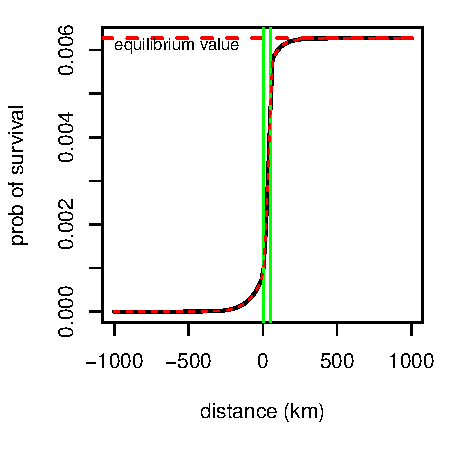
\includegraphics{prob-estab-62}
    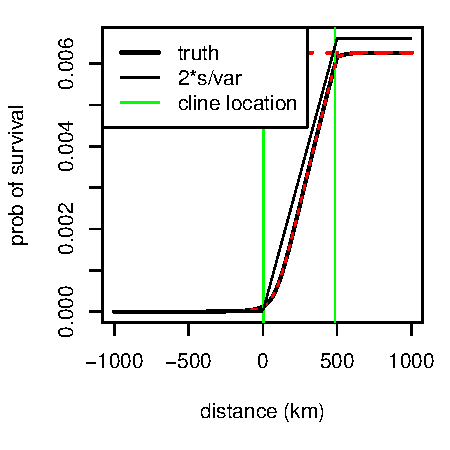
\includegraphics{prob-estab-500}
  \end{center}
  \caption{
  \plr{make this look better}
  Probability of establishment, as a function of distance along and around an altitudinal cline, whise boundaries are marked by the green lines.
  {\bf (A)} The parameters above; with cline width 62km; {\bf (B)} the same, except with cline width 500km.
  \label{sfig:prob_estab}
  }
\end{figure}


%%%%%%%
\section{Adaptation by mutation}

\plr{just a placeholder for now; to be merged in}

First, we'd like to compute how difficult is it for the beneficial adaptation to arise by new mutation.
The rate of appearance of mutant alleles is a Poisson process,
and we can assume that each is successful or not independently,
so the time until the new mutant appears and fixes is exponentially distributed,
with rate equal to the mutation rate multiplied by the probability of establishment integrated over the population.
Referring to figure~\ref{sfig:prob_estab},
we see that this is pretty close to ( (area of high altitude) $+$ ($1/2$ area of altitudial gradient) ) $\times$ (population density) $\times$ (prob of establishment at high altitude).

Let $A$ denote (area of high altitude) plus ($1/2$ area of altitudial gradient).
The population density $\rho$ is roughly 0.5--5 people per km$^2 \times$ (0.5 ha field/person) $\times$ ($2\times10^4$ plants per field ha) $=$ (5000--50000 plants per km$^2$).
As a check, the other set of numbers was ``one village per 15 km''; i.e.\ per square with 15km on a side, which is 0.444 people per km$^2$.

Since the probability of establishment at high altitude is approximately $2 s_b / \xi^2$, 
with $\xi^2$ the variance in offspring number,
the rate of appearance is just 
\begin{align*}
  \mutrate = 2 \rho A s_b \mu / \xi^2 .
\end{align*}
% rho <- 5000; sb <- 10^(-(1:3)); xisq <- 50; A <- 500
% sapply( c(1e-8,1e-5), function (mu) 2 * rho * A * sb *mu / xisq )
At the values above, with $.1 \le s_b \le .001$, the factor $2 \rho A s_b / \xi^2$ multiplying the mutation rate
varies between $10^2$ and $10^5$,
implying that a single-base mutation with $\mu=10^{-8}$ would have to wait between $10^4$ and $10^6$ generations to fix,
but a mutation with a larger target, say $\mu=10^{-5}$, would fix in tens to thousands of generations, depending on the selection coefficient.



%%%%%%%
\section{Adaptation by migration}

As we show in \jri{insert citation to theory paper} , 
the rate of adaptation by diffusive migration is roughly
\begin{align*}
  \migrate = \rho \frac{s_b \sqrt{2 s_m}}{2\xi^2} \exp\left(- \frac{\sqrt{2 s_m}R}{\sigma} \right) .
\end{align*}

\jri{do we need to expland? not sure. }
%But for now, let's interpret.

First note that for $10^{-1} \le s_m \le 10^{-4}$, the value $1/\sqrt{2s_m}$ is between 2 and 70 --
so the exponential decay of the chance of migration falls off on a scale of between 2 and 70 times the dispersal distance.
Above we have estimated the dispersal distance to be $\sigma \approx 2$ km,
and far below the mean distance $\sigma_s$ to the field that a farmer replants seed from, when this happens,
which we have as $\sigma_s = 50$ km.
Taking $\sigma=2$ km, we have that $4 \le \sigma/\sqrt{2s_m} \le 150$ km.
A very conservative upper bound might be $\sigma \le \sigma_s/20$ (if farmers replaced 10\% of their seed with long-distance seed every year).
At this upper bound, we would have $5 \le \sigma/\sqrt{2s_m} \le 175$ km,
which is not very different.
This makes the exponential term very small since $R$ is on the order of 1,000 km.

Taking $\sigma=2$ km, we then compute that 
% rho <- 5000; sb <- .01; sm <- 10^(-(1:4)); xisq <- 50; sigma <- 2
% sapply( 1000*(1:4), function (R) rho * sb * sqrt(2*sm) / (2 *  xisq) * exp(- sqrt(2*sm)*R/sigma ) )
if $s_m = 10^{-4}$ (very weak selection in the lowlands), then for $R=1,000$ km, the migration rate is $\migrate \le 10^{-5}$,
i.e.\ it would take on the order of 100,000 generations (years) to get a successful migrant only 1,000 km away,
under this model of undirected, diffusive dispersal.
For larger $s_m$, the migration rate is much smaller.

%%%%%%%%%%%%
\section{Conclusion}

It seems unlikely that any alleles that are adaptive in the highlands and deleterious at all in the lowlands
would have transited central America by undirected (diffusive) sharing of seed.
The conclusions could change if we drastically underestimate the rate of very long distance sharing of seed,
e.g.\ if sharing across hundreds of kilometers was common at some point.

Both calculations are very pessimistic about the chance of shared single-base changes through either migration or independent mutation.
However, independent mutations could be expected in kilobase-size targets,
suggesting there might be signal for genes that share adaptive changes.







\newpage
\renewcommand{\thefigure}{A\arabic{figure}}
\renewcommand{\thetable}{A\arabic{table}}

\section*{Appendix} %\label{apx:demographic_model}

\section*{Demographic modeling}

Throughout we use in many ways the {\em branching process approximation} -- if an allele is locally rare, then for at least a few generations, the fates of each offspring are nearly independent.
So, if the allele is locally deleterious, the total numbers of that allele behave as a subcritical  branching process, destined for ultimate extinction.
On the other hand, if the allele is advantageous, it will either die out or become locally common, with its fate determined in the first few generations.
If the number of offspring of an individual with this allele is the random variable $X$, 
with mean $\E[X] = 1+s$ (selective advantage $s>0$), variance $\var[X]=\xi^2$, and $\P\{X=0\}>0$ (some chance of leaving no offspring),
then the probability of local nonextinction $p_*$ is approximately $p_* \approx 2s/\xi^2$ to a second order in $s$.
The precise value can be found by defining the generating function $\Phi(u) = \E[u^X]$; 
the probability of local nonextinction $p_*$ is the minimal solution to $\Phi(1-u) = 1-u$.
(This can be seen because: $1-p_*$ is the probability that an individual's family dies out;
this is equal to the probability that the families of all that individuals' children die out;
since each child's family behaves independently, if the individual has $x$ offspring, this is equal to $(1-p_*)^x$;
and $\Phi(1-p_*) = \E[(1-p_*)^X]$.)

If the selective advantage ($s$) depends on geographic location, 
a similar fact holds: index spatial location by $i \in 1, \ldots, n$,
and for $u = (u_1,u_2,\ldots,u_n)$ define the functions $\Phi_i(u) = \E[ \prod_j u_j^{X_{ij}} ]$,
where $X_{ij}$ is the (random) number of offspring that an individual at $i$ produces at location $j$.
Then $p_* = (p_{*1}, \ldots, p_{*n})$, the vector of probabilities that a new mutation at each location eventually fixes,
is the minimal solution to $\Phi(1-p_*) = 1-p_*$,
i.e.\ $\Phi_i(1-p_*) = 1-p_{*i}$.

%%%%% in rcode/maize_calcs.R
% # maize
% N <- 103359  # plants per field
% Nf <- 561    # ears to make next generation
% e <- 0.068   # prob of total seed stock replacement
% mg <- .0083  # pollen migration
% pm <- .02    # prob of partial stock addition
% m <- 0.2     # proportion of stock replaced
% eqvals <- c(1, iterroot( function (p) { 
%             p.dead <- e + (1/2)*(1-e)*(1-Nf/N)
%             return( p.dead * 1 + 
%                     (1/2)*(1-e)*exp(((1+sb)/p.dead)*( p - 1 )) + 
%                     ((1/2)*(1-e)*Nf/N)*exp(((N/Nf)*(1+sb)/(1-e))*( p - 1 )) 
%                 )
%         } ) )
% genfn <- function (f,selx,migr=.5) { 
%         (e + (1/2)*(1-e)*(1-Nf/N))* 1 + #  no offspring
%         (1/2)*(1-e)*exp(((1+selx)/(1-e))*( f + migr*diff(c(eqvals[1],f,eqvals[2]),differences=2) - 1 )) + # pollen, Poisson mean 1+s(x)
%         (1/2)*(1-e)*(Nf/N)*exp(((N/Nf)*(1+selx/(1-e)))*( f + migr*diff(c(eqvals[1],f,eqvals[2]),differences=2) - 1 )) # seed, Poisson mean (1+s(x))*N/Nf
%     }

Here we consider a linear habitat, so that the selection coefficient at location $\ell_i$ is $s_i = \min( s_b, \max( - s_d, \alpha \ell_i ) )$.
There does not seem to be a nice analytic expression for $p_*$ in this case,
but since $1-p_*$ is a fixed point of $\Phi$, the solution can be found by iteration:
$1-p_* = \lim_{n \to \infty} \Phi^n(u)$ for an appropriate starting point $u$.

\subsection*{Maize model}

The migration and reproduction dynamics we use are taken largely from \citet{vanHeerwaarden2010}.  
On a large scale,
fields of $N$ plants are replanted each year from $N_f$ ears,
either from completely new stock (with probability $p_e$),
from partially new stock (a proportion $r_m$ with probability $p_m$),
or entirely from the same field.
Plants have an average of $\mu_E$ ears per plant, and ears have an average of $N/N_f$ kernels; 
so a plant has on average $\mu_E N/N_f$ kernels, and a field has on average $\mu_E N$ ears and $\mu_E N^2/N_f$ kernels. \jri{what happens if we change mean ears per plant from 3 to 1?}
We suppose that a plant with the selected allele is pollen parent to $(1+s) \mu_E N/N_f$ kernels,
and also seed parent to $(1+s)\mu_E N/N_f$ kernels, still in $\mu_E$ ears.
The number of offspring a plant has depends on how many of its offspring kernels get replanted.
Some proportion $m_g$ of the pollen-parent kernels are in other fields, and may be replanted;
but with probability $p_e$ no other kernels (i.e.~those in the same field) are replanted.
Otherwise, with probability $1-p_m$ the farmer chooses $N_f$ of the ears from this field to replant
(or, $(1-r_m) N_f$ of them, with probability $p_m$);
this results in a mean number $N_f/N$ (or, $(1-r_m)N_f/N$) of the plant's ears of seed children being chosen,
and a mean number $1+s$ of the plant's pollen children kernels being chosen.
Furthermore, the field is used to completely (or partially) replant another's field with chance $p_e/(1-p_e)$ (or $p_m$);
resulting in another $N_f/N$ (or $r_m N_f/N$) ears and $1+s$ (or $r_m (1+s)$) pollen children being replanted elsewhere.
Here we have assumed that pollen is well-mixed within a field,
and that the selected allele is locally rare.
Finally, we must divide all these offspring numbers by 2,
since we look at the offspring carrying a particular haplotype, not of the diploid plant's genome.

The above gives mean values; to get a probability model we assume that every count is Poisson.
In other words, we suppose that the number of pollen children is Poisson with random mean $\lambda_P$,
and the number of seed children is a mixture of $K$ independent Poissons with mean $(1+s)N/N_f$ each,
where $K$ is the random number of ears chosen to replant, which is itself Poisson with mean $\mu_K$.
By Poisson additivity, the numbers of local and migrant offspring are Poisson,
with means $\lambda_P = \lambda_{PL} + \lambda_{PM}$ and $\mu_K = \mu_{KL} + \mu_{KM}$ respectively.
With probability $p_e$, $\lambda_{PM} = m_g(1+s)$ and $\mu_K = \lambda_{PL} = 0$.
Otherwise, with probability $(1-p_e)(1-p_m)$, $\mu_{KL} = N_f/N$ and $\lambda_{PL} = (1+s)(1-m_g)$;
and with probability $(1-p_e)p_m$, $\mu_{KL} = (1-r_m) N_f/N$ and $\lambda_{PL} = (1-r_m)(1+s)(1-m_g)$.
The migrant means are,
with probability $(1-p_e) p_e/(1-p_e) = p_e$, $\mu_{KM} = N_f/N$ and $\lambda_{PM} = 1+s$;
while with probability $(1-p_e) p_m$, $\mu_{KM} = r_m N_f/N$ and $\lambda_{PM} = (1+s)(r_m(1-m_g) + m_g)$,
and otherwise $\mu_{KM} = 0$ and $\lambda_{PM} = m_g(1+s)$.


\begin{table}[htb!!]
  \begin{center}
  \begin{tabular}{|cll|}
    \hline
    complete seed stock replacement prob & $p_e$     & 0.068 \\
    pollen migration rate                & $m_g$      & 0.0083 \\
    number of plants per field           & $N$        & $10^5$ \\
    number of ears used to replant       & $N_f$      & 561 \\
    mean ears per plant                  & $\mu_E$    & 3 \\
    partial stock replacement prob       & $p_m$      & 0.02 \\
    mean proportion stock replaced       & $r_m$      & 0.2 \\
    pollen migration distance            & $\sigma_p$ & 0 km \\
    seed replacement distance            & $\sigma_s$ & 50 km \\
    distance between demes               & $a$        & 15 km \\
    width of altitudinal cline           & $w$        & 62km \\
    deleterious selection coefficient    & $s_d$      & varies \\
    beneficial selection coefficient     & $s_b$      & varies \\
    slope of selection gradient          & $\alpha$   & $(s_d+s_b)/w$ \\
    variance in offspring number         & $\xi^2$    & varies \\
    maize population density             & $\rho$     & $5 \times 10^3$ \\
    area of highland habitat             & $A$        & 500 km$^2$ \\
    mean dispersal distance              & $\sigma$   & 1.8 km \\
    \hline 
  \end{tabular}
\end{center}
  \caption{Parameter estimates used in calculations, and other notation.
  \label{tab:parameters}
  }
\end{table}


\subsection*{Math}

The generating function of a Poisson with mean $\lambda$ is $\phi(u;\lambda)=\exp(\lambda(u-1))$,
and the generating function of a Poisson($\mu$) sum of Poisson($\lambda$) values is $\phi(\phi(u;\lambda);\mu)$.
Therefore, the generating function for the diploid process, ignoring spatial structure,
is
\begin{align}
 \Phi(u) &= \begin{aligned}[t]
   & p_e \phi(u;m_g(1+s)) \\
   & \quad {} + \left\{ (1-p_e) (1-p_m) \phi(u;(1+s)(1-m_g))\phi(\phi(u;(1+s)N/N_f);N_f/N) \right. \\
   & \quad \qquad \left. {} + (1-p_e) p_m \phi(u;(1+s)(1-r_m)(1-m_g)) \phi(\phi(u;(1+s)N/N_f);(1-r_m)N_f/N) \right\} \\
   & \quad \quad {} \times \left\{ p_e/(1-p_e) \phi(u;1+s) \phi(\phi(u;(1+s)N_f/N);N_f/N) \right. \\
   & \quad \qquad \left. {} + p_m \phi(u;(1+s)(r_m(1-p_e)(1-m_g)+m_g)) \right. \\ 
   & \quad \qquad \quad \left. {}\times \phi(\phi(u;(1+s)N/N_f);r_m N_f/N)\right. \\
   & \quad \qquad \left. {} + (1 - p_e/(1-p_e)-p_m) \phi(u;m_g(1+s)) \right\}
 \end{aligned} \label{eqn:genfn} \\
 &= \begin{aligned}[t]
   & \phi(u;m_g(1+s)) \big( \; p_e \big.\\
   & \quad {} + \left\{ (1-p_e) (1-p_m) \phi(u;(1+s)(1-m_g))\phi(\phi(u;(1+s)N/N_f);N_f/N) \right. \\
   & \quad \qquad \left. {} + (1-p_e) p_m \phi(u;(1+s)(1-r_m)(1-m_g)) \phi(\phi(u;(1+s)N/N_f);(1-r_m)N_f/N) \right\} \\
   & \quad \quad {} \times \left\{ p_e/(1-p_e) \phi(u;(1+s)(1-m_g)) \phi(\phi(u;(1+s)N_f/N);N_f/N) \right. \\
   & \quad \qquad {} + p_m \phi(u;(1+s)r_m(1-m_g)) \\
   & \quad \qquad \quad {} \times \phi(\phi(u;(1+s)N/N_f);r_m N_f/N) \\
   & \quad \qquad \left. {} + (1-p_e/(1-p_e)-p_m) \right\}  \big)
 \end{aligned}
\end{align}
To get the generating function for a haploid, replace every instance of $1+s$ by $(1+s)/2$.

As a quick check,
% \begin{align}
%   \Phi(0) &= p_e + \left\{ (1-p_e)(1-p_m)+(1-p_e)p_m \right\}
%     \times \left\{ p_e/(1-p_e) + p_m + (1-p_e/(1-p_e)-p_m) \right\}
%   &= p_e + (1-p_e)
%   &= 1 .
% \end{align}
% And, 
the mean total number of offspring of a diploid is
\begin{align}
  & \begin{aligned}
(1+s) \big(
    m_g
    + & (1-p_e)\left\{ (1-p_m) ( (1-m_g) + 1 ) + p_m ( (1-r_m)(1-m_g) + (1-r_m) ) \right\} \\
    & \qquad + \left\{ p_e ( (1-m_g) + 1 ) + p_m (1-p_e)( r_m(1-m_g) + r_m ) \right\} 
    \big) 
  \end{aligned}  \\
& \qquad = 
    (1+s) \big( m_g + 
      (1-p_e)(2-m_g)(1 - p_m r_m)
      + ( p_e (2-m_g) + p_m r_m (1-p_e)(2-m_g) )
    \big) \\
& \qquad = (1+s) \big( 
    m_g + (2-m_g) ( (1-p_e) (1 - p_m r_m) + p_e + p_m r_m(1-p_e) )
  \big) \\
& \qquad = (1+s) \big( 
    m_g + (2-m_g)
  \big) \\
& \qquad = 2(1+s) .
\end{align}
\plr{CHECK}

We show numerically later that the probability of establishment is very close to $2s$ over the variance in reproductive number (as expected).
It is possible to write down an expression for the variance, but it's a big, ugly one that doesn't lend itself to intuition.

\subsection*{Migration and spatial structure}

To incorporate spatial structure, suppose that the locations $\ell_k$ are arranged in a regular grid, so that $\ell_k = a k$. 
Recall that $s_k$ is the selection coefficient at location $k$.
If the total number of offspring produced by an individual at $\ell_i$ is Poisson($\lambda_i$), with each offspring independently migrating to location $j$
with probability $m_{ij}$,
then the number of offspring at $j$ is Poisson($m_{ij}\lambda_i$),
and so the generating function is
\begin{align}
  \phi(u;\lambda,m) &= \prod_j \exp( \lambda_i m_{ij} ( u_j - 1 ) ) \\
  &= \exp\left\{ \lambda_i \left(\left(\sum_j m_{ij} u_j\right) - 1\right) \right\} .
\end{align}
We can then substitute this expression into equation \eqref{eqn:genfn},
with appropriate migration kernels for pollen and seed dispersal.

For migration, we need migration rates and migration distances for both wind-blown pollen
and for farmer seed exchange.
The rates are parameterized as above;
we need the typical dispersal distances, however.
One option is to say that the typical distance between villages is $d_v$,
and that villages are discrete demes,
so that pollen stays within the deme (pollen migration distance 0)
and seed is exchanged with others from nearby villages;
on average $\sigma_s$ distance away in a random direction.
The number of villages away the seed comes from could be geometric 
(including the possibility of coming from the same village).

\subsection{Dispersal distance}

The dispersal distance
-- the mean distance between parent and offspring --
is the average of the pollen and seed mean dispersal distances.
With the above assumptions, the pollen dispersal distance is zero,
and the seed dispersal distance is the chance of inter-village movement
multiplied by the mean distance moved.
This is
% pe <- .068; pm <- .02; rm <- .2; sigma.s <- 50
% (1/2) * (pe + (1-pe)*pm*rm) * sigma.s
\begin{align}
  \sigma = \frac{1}{2} (p_e + (1-p_e) p_m r_m ) \sigma_s = 1.7932 \text{km}
\end{align}
at the parameter values above.

Iterating the generating function above finds the probability of establishment as a function of distance along the cline.
This is shown in figure \ref{sfig:prob_estab}.
Note that the approximation $2s$ divided by the variance in offspring number is quite close.

\begin{figure}[ht!!]
  \begin{center}
    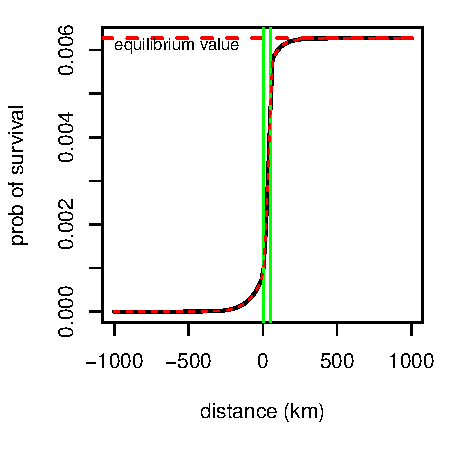
\includegraphics{prob-estab-62}
    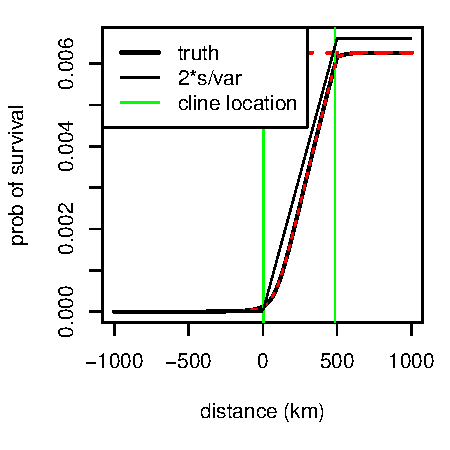
\includegraphics{prob-estab-500}
  \end{center}
  \caption{
  \plr{make this look better}
  Probability of establishment, as a function of distance along and around an altitudinal cline, whose boundaries are marked by the green lines.
  {\bf (A)} The parameters above; with cline width 62km; {\bf (B)} the same, except with cline width 500km.
  \label{sfig:prob_estab}
  }
\end{figure}


As we show in \citet{ralph2014convergent}, 
the rate of adaptation by diffusive migration is roughly
\begin{align*}
  \migrate = \rho \frac{s_b \sqrt{2 s_m}}{2\xi^2} \exp\left(- \frac{\sqrt{2 s_m}R}{\sigma} \right) .
\end{align*}

\jri{do we need to expland? not sure. }
%But for now, let's interpret.

First note that for $10^{-1} \le s_m \le 10^{-4}$, the value $1/\sqrt{2s_m}$ is between 2 and 70 --
so the exponential decay of the chance of migration falls off on a scale of between 2 and 70 times the dispersal distance.
Above we have estimated the dispersal distance to be $\sigma \approx 2$ km,
and far below the mean distance $\sigma_s$ to the field that a farmer replants seed from, when this happens,
which we have as $\sigma_s = 50$ km.
Taking $\sigma=2$ km, we have that $4 \le \sigma/\sqrt{2s_m} \le 150$ km.
A very conservative upper bound might be $\sigma \le \sigma_s/20$ (if farmers replaced 10\% of their seed with long-distance seed every year).
At this upper bound, we would have $5 \le \sigma/\sqrt{2s_m} \le 175$ km,
which is not very different.
This makes the exponential term very small since $R$ is on the order of 1,000 km.

Taking $\sigma=2$ km, we then compute that 
% rho <- 5000; sb <- .01; sm <- 10^(-(1:4)); xisq <- 50; sigma <- 2
% sapply( 1000*(1:4), function (R) rho * sb * sqrt(2*sm) / (2 *  xisq) * exp(- sqrt(2*sm)*R/sigma ) )
if $s_m = 10^{-4}$ (very weak selection in the lowlands), then for $R=1,000$ km, the migration rate is $\migrate \le 10^{-5}$,
i.e.\ it would take on the order of 100,000 generations (years) to get a successful migrant only 1,000 km away,
under this model of undirected, diffusive dispersal.
For larger $s_m$, the migration rate is much smaller.

%below moved from methods.`
If highland alleles are neutral in the lowlands the situation is more difficult to model, but we can make some informed guesses.
For maize in the Andean highlands to have inherited a highland-adapted allele from the Mexican highlands, those Andean plants must be directly descended from highland Mexican plants that lived more recently than the appearance of the adaptive allele.
In other words, the ancestral lineages along which the modern Andean plants have inherited at that locus must trace back to the Mexican highlands.
If the allele is neutral in the lowlands, we can treat the movement of these lineages as a neutral process, using the framework of coalescent theory \citep{wakeley2005coalescent}.
To do this, we need to follow \emph{all} of the $N \approx 2.5 \times 10^6$ lineages backwards; these quickly coalesce to fewer $m$ lineages in approximately $\sum_{k=m}^N \frac{2N}{\xi^2 k(k+1)} \approx 1.25 \times 10^5/m$ generations, leaving about 1000 lineages after 100 generations that are spread over a larger area.
The displacement of a lineage after $m$ generations has variance $m \sigma^2$ and is approximately Gaussian.
If we assume that $n$ lineages are independent, and $Z_n$ is the distance to the furthest lineage, then $\P\{ Z_n / \sqrt{m \sigma^2} \le x /\sqrt{2 \log n} + \sqrt{2 \log n} - (1/2) (\log \log n + \log 4 \pi)/\sqrt{2 \log n} \} \approx \exp( - e^{-x} )$ \citep{berman1964limit}. \jri{Peter are the braces in the right place? seems to me naively it should be  $\P\{ Z_n / \sqrt{m \sigma^2} \le x \} = \sqrt{2 \log n} + ...$ ??}

%%%%%%%
\section{Adaptation by mutation}

\plr{just a placeholder for now; to be merged in}

First, we'd like to compute how difficult is it for the beneficial adaptation to arise by new mutation.
The rate of appearance of mutant alleles is a Poisson process,
and we can assume that each is successful or not independently,
so the time until the new mutant appears and fixes is exponentially distributed,
with rate equal to the mutation rate multiplied by the probability of establishment integrated over the population.
Referring to figure~\ref{sfig:prob_estab},
we see that this is pretty close to ( (area of high altitude) $+$ ($1/2$ area of altitudinal gradient) ) $\times$ (population density) $\times$ (prob of establishment at high altitude).

Let $A$ denote (area of high altitude) plus ($1/2$ area of altitudinal gradient).
The population density $\rho$ is roughly 0.5--5 people per km$^2 \times$ (0.5 ha field/person) $\times$ ($2\times10^4$ plants per field ha) $=$ (5000--50000 plants per km$^2$).
As a check, the other set of numbers was ``one village per 15 km''; i.e.\ per square with 15km on a side, which is 0.444 people per km$^2$.

Since the probability of establishment at high altitude is approximately $2 s_b / \xi^2$, 
with $\xi^2$ the variance in offspring number,
the rate of appearance is just 
\begin{align*}
  \mutrate = 2 \rho A s_b \mu / \xi^2 .
\end{align*}
% rho <- 5000; sb <- 10^(-(1:3)); xisq <- 50; A <- 500
% sapply( c(1e-8,1e-5), function (mu) 2 * rho * A * sb *mu / xisq )
At the values above, with $.1 \le s_b \le .001$, the factor $2 \rho A s_b / \xi^2$ multiplying the mutation rate
varies between $10^2$ and $10^5$,
implying that a single-base mutation with $\mu=10^{-8}$ would have to wait between $10^4$ and $10^6$ generations to fix,
but a mutation with a larger target, say $\mu=10^{-5}$, would fix in tens to thousands of generations, depending on the selection coefficient.



%%%%%%%
\section{Adaptation by migration}

%%%%%%%%%%%%
\section{Conclusion}
It seems unlikely that any alleles that are adaptive in the highlands and deleterious at all in the lowlands
would have transited central America by undirected (diffusive) sharing of seed.
The conclusions could change if we drastically underestimate the rate of very long distance sharing of seed,
e.g. if sharing across hundreds of kilometers was common at some point.

Both calculations are very pessimistic about the chance of shared single-base changes through either migration or independent mutation.
However, independent mutations could be expected in kilobase-size targets,
suggesting there might be signal for genes that share adaptive changes.


\newpage
\suppl
\section*{Supporting information}

\newpage

%\clearpage

% space of double hline in Table
\doublerulesep = 0.4pt

%\section*{SUPPLEMENTAL METHODS}
\renewcommand{\thefigure}{S\arabic{figure}}
\renewcommand{\thetable}{S\arabic{table}}


%%%%%%%%%%%%%%%%%%%%%%%%%%%%%%%
%Table S1 %
\renewcommand{\arraystretch}{1.2}

\begin{table}[h]
    \begin{center}
    \caption[]{List of maize landraces used in this study\hspace*{9.1cm}}  
{\fontsize{7}{10}\selectfont
%{\small
    \begin{tabular}{llllllllll}
        \hline\hline
       & & & \\[-4mm] 
	 ID$^a$	&	USDA ID	&	Population	&	Landrace	&	Locality	&	Latitude	&	Longitude	&	Elevation	&	Origin	\\[0.0cm]
	\hline 
	& & & \\[-4mm] 
{\bf RIMMA0409}	&	PI 478968	&	Mexico 	&	Tepecintle	&	Chiapas, Mexico	&	15.4 	&	-92.9 	&	107	&	USDA	\\
RIMMA0410	&	PI 478970	&	Lowland	&	Vandeno	&	Chiapas, Mexico	&	15.4 	&	-92.9 	&	107	&	USDA	\\
{\bf RIMMA0433}	&	PI 490825	&		&	Nal Tel ATB	&	Chiquimula, Guatemala	&	14.7 	&	-89.5 	&	457	&	USDA	\\
{\bf RIMMA0441}	&	PI 515538	&		&	Coscomatepec	&	Veracruz, Mexico	&	19.2 	&	-97.0 	&	1320	&	USDA	\\
{\bf RIMMA0615}	&	PI 628480	&		&	Tuxpeno	&	Puebla, Mexico	&	20.1 	&	-97.2 	&	152	&	USDA	\\
{\bf RIMMA0619}	&	PI 645772	&		&	Pepitilla	&	Guerrero, Mexico	&	18.4 	&	-99.5 	&	747	&	USDA	\\
{\bf RIMMA0628}	&	PI 646017	&		&	Tuxpeno Norteno	&	Tamaulipas, Mexico	&	23.3 	&	-99.0 	&	300	&	USDA	\\
{\bf RIMMA0696}	&	Ames 28568	&		&	Tuxpeno	&	El Progreso, Guatemala	&	16.5 	&	-90.2 	&	30	&	Goodman	\\
{\bf RIMMA0700}	&	NSL 291626	&		&	Olotillo	&	Chiapas, Mexico	&	16.8 	&	-93.2 	&	579	&	Goodman	\\
{\bf RIMMA0701}	&	PI 484808	&		&	Olotillo	&	Chiapas, Mexico	&	16.6 	&	-92.7 	&	686	&	Goodman	\\
{\bf RIMMA0702}	&	Ames 28534	&		&	Negro de Tierra Caliente	&	Sacatepequez, Guatemala	&	14.5 	&	-90.8 	&	1052	&	Goodman	\\
{\bf RIMMA0703}	&	NSL 283390	&		&	Nal Tel	&	Yucatan, Mexico	&	20.8 	&	-88.5 	&	30	&	Goodman	\\
{\bf RIMMA0709}	&	Ames 28452	&		&	Tehua	&	Chiapas, Mexico	&	16.5 	&	-92.5 	&	747	&	Goodman	\\
{\bf RIMMA0710}	&	PI 478988	&		&	Tepecintle	&	Chiapas, Mexico	&	15.3 	&	-92.6 	&	91	&	Goodman	\\
{\bf RIMMA0712}	&	NSL 291696 CYMT	&		&	Oloton	&	Baja Verapaz, Guatemala	&	15.3 	&	-90.3 	&	1220	&	Goodman	\\
{\bf RIMMA0716}	&	Ames 28459	&		&	Zapalote Grande	&	Chiapas, Mexico	&	15.3 	&	-92.7 	&	91	&	Goodman	\\
{\bf RIMMA0720}	&	PI 489372	&		&	Negro de Tierra Caliente	&	Guatemala	&	15.5 	&	-88.9 	&	39	&	Goodman	\\
{\bf RIMMA0721}	&	Ames 28485	&		&	Nal Tel ATB	&	Chiquimula, Guatemala	&	14.6 	&	-90.1 	&	915	&	Goodman	\\
{\bf RIMMA0722}	&	Ames 28564	&		&	Dzit Bacal	&	Jutiapa, Guatemala	&	14.3 	&	-89.7 	&	737	&	Goodman	\\
{\bf RIMMA0727}	&	Ames 28555	&		&	Comiteco	&	Guatemala	&	14.4 	&	-90.5 	&	1151	&	Goodman	\\
{\bf RIMMA0729}	&	PI 504090	&		&	Tepecintle	&	Guatemala	&	15.4 	&	-89.7 	&	122	&	Goodman	\\
{\bf RIMMA0730}	&	Ames 28517	&		&	Quicheno Late	&	Sacatepequez, Guatemala	&	14.5 	&	-90.8 	&	1067	&	Goodman	\\
{\bf RIMMA0731}	&	PI 484137	&		&	Bolita	&	Oaxaca, Mexico	&	16.8 	&	-96.7 	&	1520	&	Goodman	\\
{\bf RIMMA0733}	&	PI 479054	&		&	Zapalote Chico	&	Oaxaca, Mexico	&	16.6 	&	-94.6 	&	107	&	Goodman	\\
	\hline 
	& & & \\[-4mm] 
{\bf RIMMA0416}	&	PI 484428	&	Mexico	&	Cristalino de Chihuahua	&	Chihuahua, Mexico	&	29.4 	&	-107.8 	&	2140	&	NA	\\
{\bf RIMMA0417}	&	PI 484431	&	Highland	&	Azul	&	Chihuahua, Mexico	&	28.6 	&	-107.5 	&	2040	&	USDA	\\
{\bf RIMMA0418}	&	PI 484476	&		&	Gordo	&	Chihuahua, Mexico	&	28.6 	&	-107.5 	&	2040	&	USDA	\\
{\bf RIMMA0421}	&	PI 484595	&		&	Conico	&	Puebla, Mexico	&	19.9 	&	-98.0 	&	2250	&	USDA	\\
{\bf RIMMA0422}	&	PI 485071	&		&	Elotes Conicos	&	Puebla, Mexico	&	19.1 	&	-98.3 	&	2200	&	USDA	\\
{\bf RIMMA0423}	&	PI 485116	&		&	Cristalino de Chihuahua	&	Chihuahua, Mexico	&	29.2 	&	-108.1 	&	2095	&	NA	\\
{\bf RIMMA0424}	&	PI 485120	&		&	Apachito	&	Chihuahua, Mexico	&	28.0 	&	-107.6 	&	2400	&	USDA	\\
{\bf RIMMA0425}	&	PI 485128	&		&	Palomero Tipo Chihuahua	&	Chihuahua, Mexico	&	26.8 	&	-107.1 	&	2130	&	USDA	\\
{\bf RIMMA0614}	&	PI 628445	&		&	Mountain Yellow	&	Jalisco, Mexico	&	20.0 	&	-103.8 	&	2060	&	USDA	\\
{\bf RIMMA0616}	&	PI 629202	&		&	Zamorano Amarillo	&	Jalisco, Mexico	&	20.8 	&	-102.8 	&	1800	&	USDA	\\
{\bf RIMMA0620}	&	PI 645786	&		&	Celaya	&	Guanajuato, Mexico	&	20.2 	&	-100.9 	&	1799	&	USDA	\\
{\bf RIMMA0621}	&	PI 645804	&		&	Zamorano Amarillo	&	Guanajuato, Mexico	&	21.1 	&	-101.7 	&	1870	&	USDA	\\
{\bf RIMMA0623}	&	PI 645841	&		&	Palomero de Jalisco	&	Jalisco, Mexico	&	20.0 	&	-103.7 	&	2520	&	USDA	\\
{\bf RIMMA0625}	&	PI 645984	&		&	Cacahuacintle	&	Puebla, Mexico	&	19.0 	&	-97.4 	&	2600	&	USDA	\\
RIMMA0626	&	PI 645993	&		&	Arrocillo Amarillo	&	Puebla, Mexico	&	19.9 	&	-97.6 	&	2260	&	USDA	\\
{\bf RIMMA0630}	&	PI 646069	&		&	Arrocillo Amarillo	&	Veracruz, Mexico	&	19.8 	&	-97.3 	&	2220	&	USDA	\\
{\bf RIMMA0670}	&	Ames 28508	&		&	San Marceno	&	San Marcos, Guatemala	&	15.0 	&	-91.8 	&	2378	&	Goodman	\\
{\bf RIMMA0671}	&	Ames 28538	&		&	Salpor Tardio	&	Solola, Guatemala	&	14.8 	&	-91.3 	&	2477	&	Goodman	\\
{\bf RIMMA0672}	&	PI 483613	&		&	Chalqueno	&	Mexico, Mexico	&	19.7 	&	-99.1 	&	2256	&	Goodman	\\
{\bf RIMMA0674}	&	PI 483617	&		&	Toluca	&	Mexico, Mexico	&	19.3 	&	-99.7 	&	2652	&	Goodman	\\
{\bf RIMMA0677}	&	Ames 28476 	&		&	Conico Norteno	&	Zacatecas, Mexico	&	21.4 	&	-102.9 	&	1951	&	Goodman	\\
{\bf RIMMA0680}	&	Ames 28448	&		&	Tabloncillo	&	Jalisco, Mexico	&	20.4 	&	-102.2 	&	1890	&	Goodman	\\
{\bf RIMMA0682}	&	PI 484571	&		&	Tablilla de Ocho	&	Jalisco, Mexico	&	22.1 	&	-103.2 	&	1700	&	Goodman	\\
{\bf RIMMA0687}	&	Ames 28473	&		&	Conico Norteno	&	Queretaro, Mexico	&	20.4 	&	-100.0 	&	1921	&	Goodman	\\[-0.1mm]	
	                         %&                       &                                 & \emph{BoS-68}  & AB298905       &  AB054737\\[-0.1mm]	
	\hline\hline
\multicolumn{9}{l}{$^a$ GBS data are available for the accessions in bold font.}\\
    \end{tabular}}

\end{center} 

\end{table}

\clearpage
%%%%%%%%%%%%%%%%%%%%%%%%%%%%%%%%%%%%%%%%%%%

\setcounter{table}{0}
%%%%%%%%%%%%%%%%%%%%%%%%%%%%%%%
%Table S1 %
\renewcommand{\arraystretch}{1.2}

\begin{table}[h]
    \begin{center}
    \caption[]{(continued)\hspace*{13.5cm}}  
{\fontsize{7}{10}\selectfont
%{\small
    \begin{tabular}{llllllllll}
        \hline\hline
       & & & \\[-4mm] 
	 ID	&	USDA ID	&	Population	&	Landrace	&	Locality	&	Latitude	&	Longitude	&	Elevation (m)	&	Origin	\\[0.0cm]
	\hline 
	& & & \\[-4mm] 
{\bf RIMMA0388}	&	PI 443820	&	S. America	&	Amagaceno	&	Antioquia, Colombia	&	6.9 	&	-75.3 	&	1500	&	USDA	\\
{\bf RIMMA0389}	&	PI 444005	&	Lowland	&	Costeno	&	Atlantico, Colombia	&	10.4 	&	-74.9 	&	7	&	USDA	\\
{\bf RIMMA0390}	&	PI 444254	&		&	Comun	&	Caldas, Colombia	&	4.5 	&	-75.6 	&	353	&	USDA	\\
RIMMA0391	&	PI 444296	&		&	Andaqui	&	Caqueta, Colombia	&	1.4 	&	-75.8 	&	700	&	USDA	\\
{\bf RIMMA0392}	&	PI 444309	&		&	Andaqui	&	Caqueta, Colombia	&	1.8 	&	-75.6 	&	555	&	USDA	\\
{\bf RIMMA0393}	&	PI 444473	&		&	Costeno	&	Cordoba, Colombia	&	8.3 	&	-75.2 	&	100	&	USDA	\\
{\bf RIMMA0394}	&	PI 444621	&		&	Pira	&	Cundinamarca, Colombia	&	4.8 	&	-74.7 	&	1000	&	USDA	\\
{\bf RIMMA0395}	&	PI 444731	&		&	Negrito	&	Choco, Colombia	&	8.5 	&	-77.3 	&	30	&	USDA	\\
{\bf RIMMA0396}	&	PI 444834	&		&	Caqueteno	&	Huila, Colombia	&	2.6 	&	-75.3 	&	1100	&	USDA	\\
{\bf RIMMA0397}	&	PI 444897	&		&	Negrito	&	Magdalena, Colombia	&	11.6 	&	-72.9 	&	50	&	USDA	\\
{\bf RIMMA0398}	&	PI 444923	&		&	Puya	&	Magdalena, Colombia	&	9.4 	&	-75.7 	&	27	&	USDA	\\
{\bf RIMMA0399}	&	PI 444954	&		&	Cariaco	&	Magdalena, Colombia	&	10.2 	&	-74.1 	&	250	&	USDA	\\
{\bf RIMMA0403}	&	PI 445163	&		&	Pira Naranja	&	Narino, Colombia	&	1.3 	&	-77.5 	&	1000	&	USDA	\\
{\bf RIMMA0404}	&	PI 445322	&		&	Puya Grande	&	Norte de Santander, Colombia	&	7.3 	&	-72.5 	&	1500	&	USDA	\\
RIMMA0405	&	PI 445355	&		&	Puya	&	Norte de Santander, Colombia	&	8.4 	&	-73.3 	&	1100	&	USDA	\\
{\bf RIMMA0406}	&	PI 445514	&		&	Yucatan	&	Tolima, Colombia	&	5.0 	&	-74.9 	&	450	&	USDA	\\
RIMMA0407	&	PI 445528	&		&	Pira	&	Tolima, Colombia	&	4.2 	&	-74.9 	&	450	&	USDA	\\
{\bf RIMMA0428}	&	PI 485354	&		&	Aleman	&	Huanuco, Peru	&	-9.3 	&	-76.0 	&	700	&	NA	\\
{\bf RIMMA0462}	&	PI 445073	&		&	Amagaceno	&	Narino, Colombia	&	1.6 	&	-77.2 	&	1700	&	USDA	\\
{\bf RIMMA0690}	&	PI 444946	&		&	Puya	&	Magdalena, Colombia	&	8.3 	&	-73.6 	&	250	&	Goodman	\\
{\bf RIMMA0691}	&	PI 445391	&		&	Cacao	&	Santander, Colombia	&	6.6 	&	-73.1 	&	1098	&	NA	\\
{\bf RIMMA0707}	&	PI 487930	&		&	Tuxpeno	&	Ecuador	&	-1.1 	&	-80.5 	&	30	&	Goodman	\\
{\bf RIMMA0708}	&	PI 488376	&		&	Yunquillano F Andaqui	&	Ecuador	&	-3.5 	&	-78.6 	&	1098	&	Goodman	\\
	\hline 
	& & & \\[-4mm] 
{\bf RIMMA0426}	&	PI 485151	&	S. America	&	Rabo de Zorro	&	Ancash, Peru	&	-9.1 	&	-77.8 	&	2500	&	NA	\\
{\bf RIMMA0430}	&	PI 485362	&	Highland	&	Sarco	&	Ancash, Peru	&	-9.2 	&	-77.7 	&	2585	&	NA	\\
{\bf RIMMA0431}	&	PI 485363	&	 	&	Perlilla	&	Huanuco, Peru	&	-8.7 	&	-77.1 	&	2900	&	NA	\\
{\bf RIMMA0436}	&	PI 514723	&		&	Morocho Cajabambino	&	Amazonas, Peru	&	-6.2 	&	-77.9 	&	2200	&	NA	\\
{\bf RIMMA0437}	&	PI 514752	&		&	Ancashino	&	Ancash, Peru	&	-9.3 	&	-77.6 	&	2688	&	NA	\\
{\bf RIMMA0438}	&	PI 514809	&		&	Maranon	&	Ancash, Peru	&	-8.7 	&	-77.4 	&	2820	&	NA	\\
RIMMA0439	&	PI 514969	&		&	Maranon	&	La Libertad, Peru	&	-8.5 	&	-77.2 	&	2900	&	NA	\\
{\bf RIMMA0464}	&	PI 571438	&		&	Chullpi	&	Huancavelica, Peru	&	-12.3 	&	-74.7 	&	1800	&	USDA	\\
{\bf RIMMA0465}	&	PI 571457	&		&	Huarmaca	&	Piura, Peru	&	-5.6 	&	-79.5 	&	2300	&	USDA	\\
{\bf RIMMA0466}	&	PI 571577	&		&	Confite Puneno	&	Apurimac, Peru	&	-14.3 	&	-72.9 	&	3600	&	USDA	\\
{\bf RIMMA0467}	&	PI 571871	&		&	Paro	&	Apurimac, Peru	&	-13.6 	&	-72.9 	&	2800	&	USDA	\\
{\bf RIMMA0468}	&	PI 571960	&		&	Sarco	&	Ancash, Peru	&	-9.4 	&	-77.2 	&	3150	&	USDA	\\
{\bf RIMMA0473}	&	PI 445114	&		&	Sabanero	&	Narino, Colombia	&	1.1 	&	-77.6 	&	3104	&	USDA	\\
{\bf RIMMA0656}	&	Ames 28799	&		&	Culli	&	Jujuy, Argentina	&	-23.2 	&	-65.4 	&	2287	&	Goodman	\\
{\bf RIMMA0657}	&	NSL 286594	&		&	Chake Sara	&	Bolivia	&	-17.5 	&	-65.7 	&	2201	&	Goodman	\\
{\bf RIMMA0658}	&	NSL 286812	&		&	Uchuquilla	&	Bolivia	&	-21.8 	&	-64.1 	&	1948	&	Goodman	\\
{\bf RIMMA0661}	&	PI 488066	&		&	Chillo	&	Ecuador	&	-2.9 	&	-78.7 	&	2195	&	Goodman	\\
{\bf RIMMA0662}	&	NSL 287008	&		&	Cuzco	&	Ecuador	&	0.0 	&	-78.0 	&	2195	&	Goodman	\\
{\bf RIMMA0663}	&	PI 488102	&		&	Mishca	&	Ecuador	&	0.4 	&	-78.2 	&	2067	&	Goodman	\\
{\bf RIMMA0664}	&	PI 488113	&		&	Blanco Blandito	&	Ecuador	&	0.4 	&	-78.4 	&	2122	&	Goodman	\\
{\bf RIMMA0665}	&	PI 489324	&		&	Racimo de Uva	&	Ecuador	&	-0.9 	&	-78.9 	&	2931	&	Goodman	\\
{\bf RIMMA0667}	&	Ames 28737	&		&	Patillo	&	Chuquisaca, Bolivia	&	-21.8 	&	-64.1 	&	2201	&	NA	\\
RIMMA0668	&	Ames 28668	&		&	Granada	&	Puno, Peru	&	-14.9 	&	-70.6 	&	3925	&	Goodman	\\[-0.1mm] 
	                         %&                       &                                 & \emph{BoS-68}  & AB298905       &  AB054737\\[-0.1mm]	
	\hline\hline
	\multicolumn{9}{l}{$^a$ GBS data are available for the accessions in bold font.}\\
    \end{tabular}}
    \label{srkid}

\end{center} 

\end{table}

\clearpage
%%%%%%%%%%%%%%%%%%%%%%%%%%%%%%%%%%%%%%%%%%%




%%%%%%%%%%%%%%%%%%%%%%%%%%%%%%%%%%%%%%%%%%%%%%%%%%%%%%%%%%%%
\renewcommand{\arraystretch}{1.1}
\begin{table}[h]

\begin{center}
 \caption[]{Inference of demographic parameters\hspace*{0.3cm}}
  \textbf{}\\[-2mm]
{\fontsize{8}{11}\sf
    \begin{tabular}{ccccccccl} \hline\hline
       & & \\[-3mm]
     Mexico  & \multicolumn{2}{c}{Model IA}  \\[0.1cm]
    \hline
    & & \\[-3mm]
   & Likelihood & $-$3052.34  \\
  &$N_B$ & 148,500 \\
  &$N_C$ & 148,500 \\   
  &$N_1$ & 62,370 \\ 
  &$N_2$ & 86,130 \\ 
  &$N_{2P}$   & 86,130    \\ 
      \hline
    & & \\[-3mm]
    S. America  & \multicolumn{2}{c}{Model IA}  \\[0.1cm]
        \hline
    & & \\[-3mm]
     & Likelihood &  $-$2717.64  \\
       &$N_B$ & 76,500 \\     	
       &$N_C$ & 76,500 \\
      &$N_1$ & 74,205           \\ 
      &$N_2$ & 2,295       \\      
      &$N_{2P}$   & 346,545   \\[1mm]
    \hline\hline
\multicolumn{3}{l}{The description of $\alpha, \beta$ and $\gamma$ is in Figure~3.}\\
\multicolumn{3}{l}{$\sigma$ is a relative size of $N_B$ to $N_C$ ($N_B=\sigma N_C$).}\\
    \end{tabular}
    \label{supp:param}  % caption is needed to make this work
}
\end{center}
\end{table}
\renewcommand{\arraystretch}{1}
%%%%%%%%%%%%%%%%%%%%%%%%%%%%%%%%%%%%%%%%%%%%%%%%%%%%%%%%%%%%


%%%%%%%%%%%%%%%%%%%%%%%%%%%%%%%%%%%%%%%%%%%%%%%%%%%%%%%%%%%%
\renewcommand{\arraystretch}{1.1}
\begin{table}[h]

\begin{center}
 \caption[]{Summary of PHS test\hspace*{6.1cm}}
  \textbf{}\\[-2mm]
{\fontsize{8}{11}\sf
    \begin{tabular}{lllllcccccl} \hline\hline
       & & \\[-3mm]
     Population  & Pattern of adaptation & No. SNPs & No. SNPs supported by PHS test \\[0.1cm]
    \hline
    & & \\[-3mm]
   Mexico & Highland adaptation & 264 & 172 (65.2\%)  \\
               & Lowland adaptation & 101 & 66 (65.3\%)  \\
   S. America & Highland adaptation & 164 & 230 (71.3\%)  \\
                     & Lowland adaptation & 70 & 50 (71.4\%)  \\[0.1cm]
    \hline\hline
    \end{tabular}
    \label{supp:phs}  % caption is needed to make this work
}
\end{center}
\end{table}
\renewcommand{\arraystretch}{1}
%%%%%%%%%%%%%%%%%%%%%%%%%%%%%%%%%%%%%%%%%%%%%%%%%%%%%%%%%%%%

%%%%%%%%%%%%%%%%%%%%%%%%%%%%%%%%%%%%%%%%%%%%%%%%%%%%%%%%%%%%
\renewcommand{\arraystretch}{1.1}
\begin{table}[h]

\begin{center}
 \caption[]{$F_{CT}$ between \emph{parviglumis} and \emph{mexicana}\hspace*{0.3cm}}
  \textbf{}\\[-2mm]
{\fontsize{7}{11}\sf
    \begin{tabular}{lcccccccl} 
    \hline\hline
       
Mexico     & \multicolumn{3}{c}{Number of SNPs}  \\
                                  & Significant & NS          & Proportion  \\
Significant $F_{CT}$ & 25              &   337       & 0.077\\ 
NS                             & 299            &  18,493   & 0.018\\
      \hline
    & & \\[-3mm]
S. America     & \multicolumn{3}{c}{Number of SNPs} \\
                                     & Significant & NS           & Proportion  \\
Significant $F_{CT}$    & 10              &   327        & 0.070\\ 
NS                                & 133            &  17,518    & 0.018\\[1mm]
    \hline\hline
  %\multicolumn{4}{l}{$^{a}$ \textcolor{red}{Maybe we should use the number of genetic unit.}}\\
  % \multicolumn{4}{l}{$^{a}$ \textcolor{red}{Sum of the number of SNPs != 91,779 because I excluded SNPs exhibiting}}\\[-0.5mm]
  % \multicolumn{4}{l}{ \textcolor{red}{     monomorphic in Mexico or in South America.}}\\
    \end{tabular}
    \label{tanja}  % caption is needed to make this work
}
\end{center}
\end{table}
\renewcommand{\arraystretch}{1}
%%%%%%%%%%%%%%%%%%%%%%%%%%%%%%%%%%%%%%%%%%%%%%%%%%%%%%%%%%%%


%%%%%%%%%%%%%%%%%%%%%%%%%%%%%%%%%%%%%%%%%%%%%%%%%%%%%%%%%%%%=
\begin{table}[h]	
	\caption[]{$F_{ST}$ outlier SNPs and \emph{mexicana} introgression\hspace*{0.3cm}} 
			\centering
			\textbf{}\\[-2mm]
			{\fontsize{7}{11}\sf
		    \begin{tabular}{llcc} \hline\hline
		    & & \\[-3mm]
		    Introgression status & Population & $F_{ST}$ outlier SNPs & All other SNPs \\
		    \hline
		   Introgressed & Mexico & 114 & 1953 \\
		 	& S. America & 26 & 1721 \\
		   Not introgressed & Mexico & 558 & 73892 \\
		 	& S. America & 379 & 60666 \\
		      \hline\hline
		    \end{tabular}
		    \label{supp:introgressed}  % caption is needed to make this work
		}
\end{table}
%%%%%%%%%%%%%%%%%%%%%%%%%%%%%%%%%%%%%%%%%%%%%%%%%%%%%%%%%%%%


%%%%%%%%%%%%%%%%%%%%%%%%%%%%%%%%%%%%%%%%%%%%%%%%%%%%%%%%%%%%
\renewcommand{\arraystretch}{1.1}
\begin{table}[h]

\begin{center}
 \caption[]{ms command \st{you don't use this table?}\hspace*{13.3cm}}
  \textbf{}\\[-2mm]
{\fontsize{7}{11}\sf
    \begin{tabular}{llcccccccl} \hline\hline
       & & \\[-3mm]
     Model I for Mexico  populations   \\
     Population 1: Mexico lowland population   \\
     Population 2: Mexico highland population   \\
  -I 2 $n_{m1}$ $n_{m2}$ -n 1 0.3496 -n 2 0.5704 -ej 0.01 2 1 -en 0.01 1 0.92 -en 0.0133 1 0.0163 -en 0.015 1 1.0 \\ 
      \hline
    & & \\[-3mm]
     Model II for Mexico  populations   \\
     Population 1: Mexico lowland population   \\
     Population 2: Mexico highland population   \\
     Population 3: \emph{mexicane} population   \\
-I 2 $n_{m1}$ $n_{m2}$ -n 1 1.14 -n 2 0.36 -es 0.01 2 0.8 -en 0.01 3 1.0667 -ej 0.01 2 1 -en 0.01 1 1.5 -en 0.0133 1 0.0163 -en 0.015 1 1.0 -ej 0.1 3 1 \\ 
      \hline
    & & \\[-3mm]
    Model I for SA  populations   \\
     Population 1: SA lowland population   \\
     Population 2: SA highland population   \\
  -I 2 $n_{s1}$ $n_{s2}$ -n 1 0.5044 -n 2 1.3728 -g 2 671.60 -ej 0.006667 2 1 -eg 0.006667 2 0.0 -en 0.00667 1 0.52 -en 0.01333 1 0.0163 -en 0.015 1 1.0 \\ 
      \hline
    & & \\[-3mm]
    Model III for SA  populations   \\
    Population 1: Mexico lowland population   \\
     Population 2: SA lowland population   \\
     Population 3: SA highland population   \\
  -I 3 $n_{m1}$ $n_{s1}$ $n_{s2}$ -n 1 0.64 -n 2 0.342 -n 3 0.972 -g 3 598.35 -ej 0.006667 3 2 -eg 0.006667 3 0.0 -en 0.006667 2 0.36 -ej 0.01 2 1\\
   -en 0.01 1 1 -en 0.0133 1 0.0163 -en 0.015 1 1.0 \\  [1mm]
    \hline\hline
\multicolumn{1}{l}{Sample size of Mexico lowland, Mexico highland, SA lowland and SA highland populations are denoted by $n_{m1}$, $n_{m2}$, $n_{s1}$ and $n_{s2}$, respectively.}\\
    \end{tabular}
    \label{commandline}  % caption is needed to make this work
}
\end{center}
\end{table}
\renewcommand{\arraystretch}{1}
%%%%%%%%%%%%%%%%%%%%%%%%%%%%%%%%%%%%%%%%%%%%%%%%%%%%%%%%%%%%

%%%%%%%%%%%%%%%%%%%%%%%%%%%%%%%%%%%%%%%%%%%%%%%%%%%%%%%%%%%%
\begin{figure}[h]
  \begin{center}
    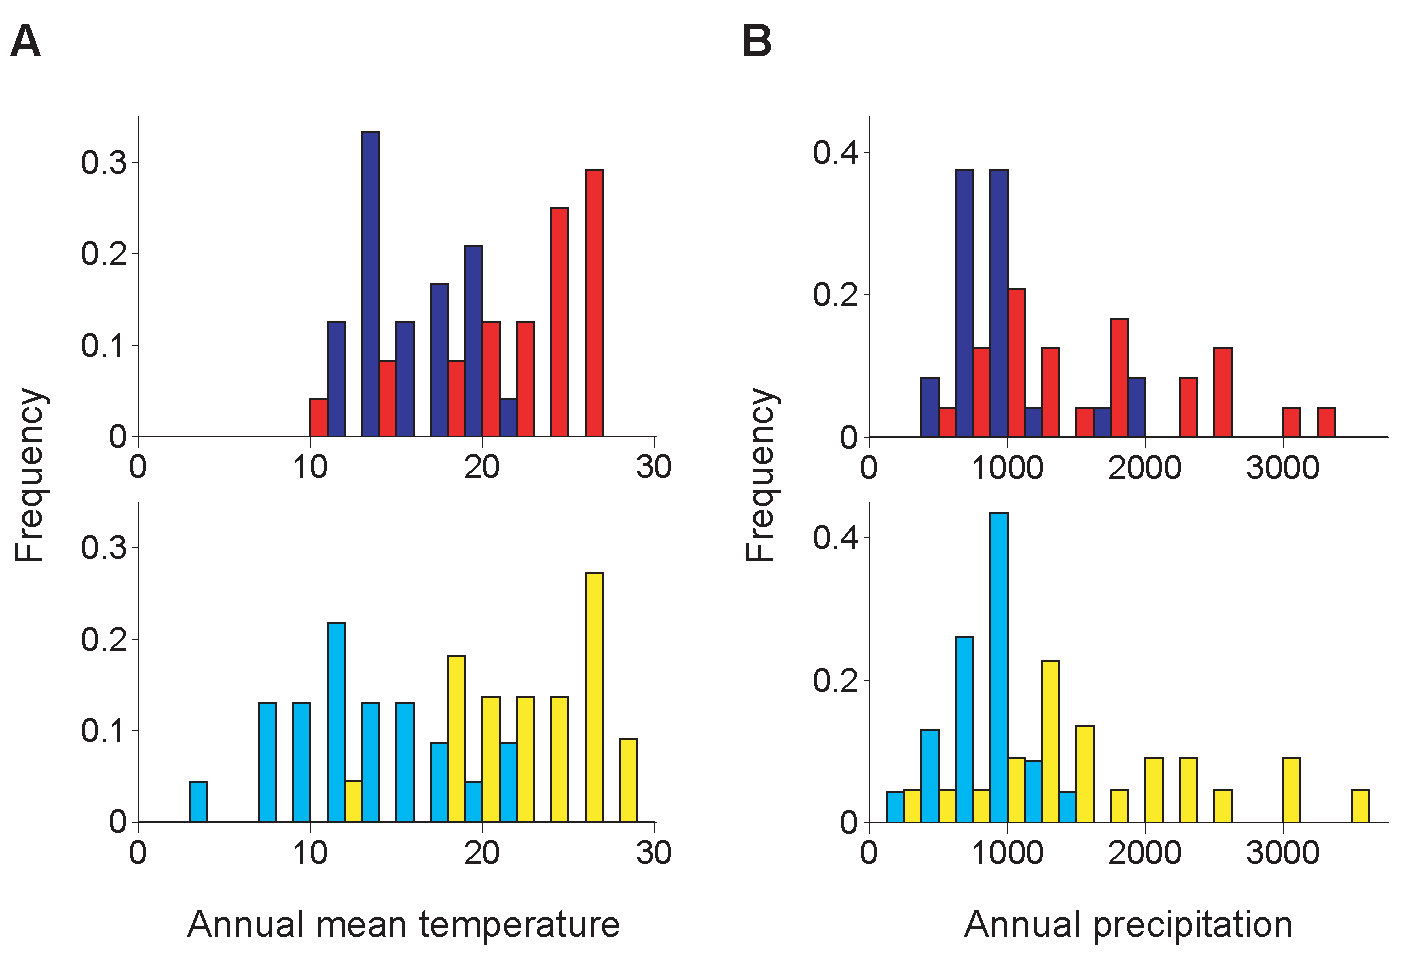
\includegraphics[width=0.5\columnwidth]{fig/bioclm.pdf}
    \caption{Annual mean temperature and annual precipitation in the sampling locations of the maize landraces across Americas.
    Red, blue, yellow and light blue bars represent Mexican lowland, Mexican highland, S. American lowland and S. American highland
    populations, respectively.  
    }
    \label{supp:colfreq}
  \end{center}
\end{figure}
%%%%%%%%%%%%%%%%%%%%%%%%%%%%%%%%%%%%%%%%%%%%%%%%%%%%%%%%%%%%

%%%%%%%%%%%%%%%%%%%%%%%%%%%%%%%%%%%%%%%%%%%%%%%%%%%%%%%%%%%%
\begin{figure}[h]
  \begin{center}
    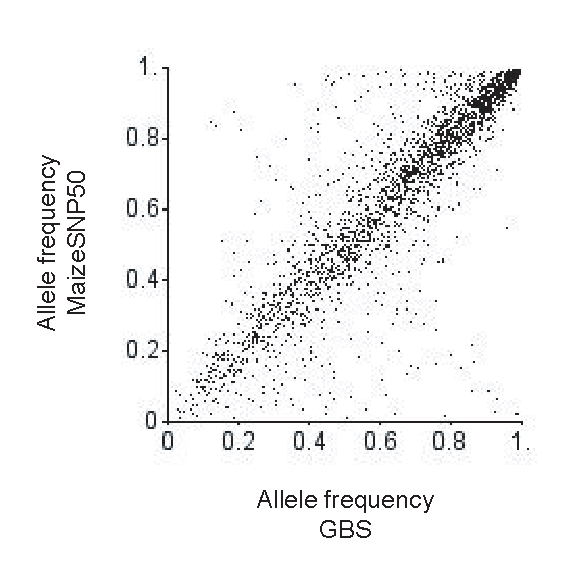
\includegraphics[width=0.4\columnwidth]{fig/Col.pdf}
    \caption{Correlation of allele frequencies between GBS (\emph{x}-axes) and MaizeSNP50 (\emph{y}-axes) data.  We used overlapped SNPs with $n\geq40$ for both data sets.  Correlation coefficient is 0.890 ($P<10^{-5}$ by permutation test with $10^5$ replications).}
    \label{supp:correl_freq}
  \end{center}
\end{figure}
%%%%%%%%%%%%%%%%%%%%%%%%%%%%%%%%%%%%%%%%%%%%%%%%%%%%%%%%%%%%

%%%%%%%%%%%%%%%%%%%%%%%%%%%%%%%%%%%%%%%%%%%%%%%%%%%%%%%%%%%%
\begin{figure}[h]
  \begin{center}
    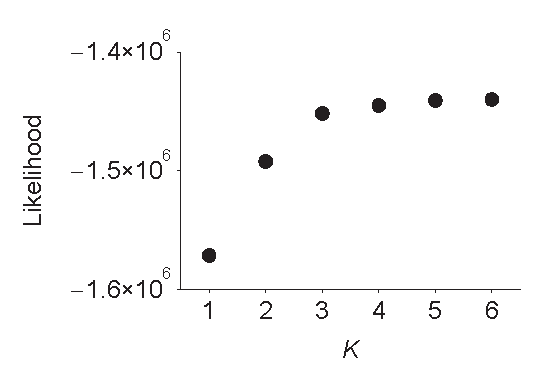
\includegraphics[width=0.4\columnwidth]{fig/kk.pdf}
    \caption{Likelihood of STRUCTURE analysis given $K$.  The \emph{x}-axes represents $K$ and the \emph{y}-axes represents likelihood.}
    \label{supp:struct}
  \end{center}
\end{figure}
%%%%%%%%%%%%%%%%%%%%%%%%%%%%%%%%%%%%%%%%%%%%%%%%%%%%%%%%%%%%

%%%%%%%%%%%%%%%%%%%%%%%%%%%%%%%%%%%%%%%%%% FIGURE
\begin{figure}[h]   
  \begin{center}
   \vspace{-0mm}
   %\includegraphics[width=0.23\textwidth]{figs/model}
   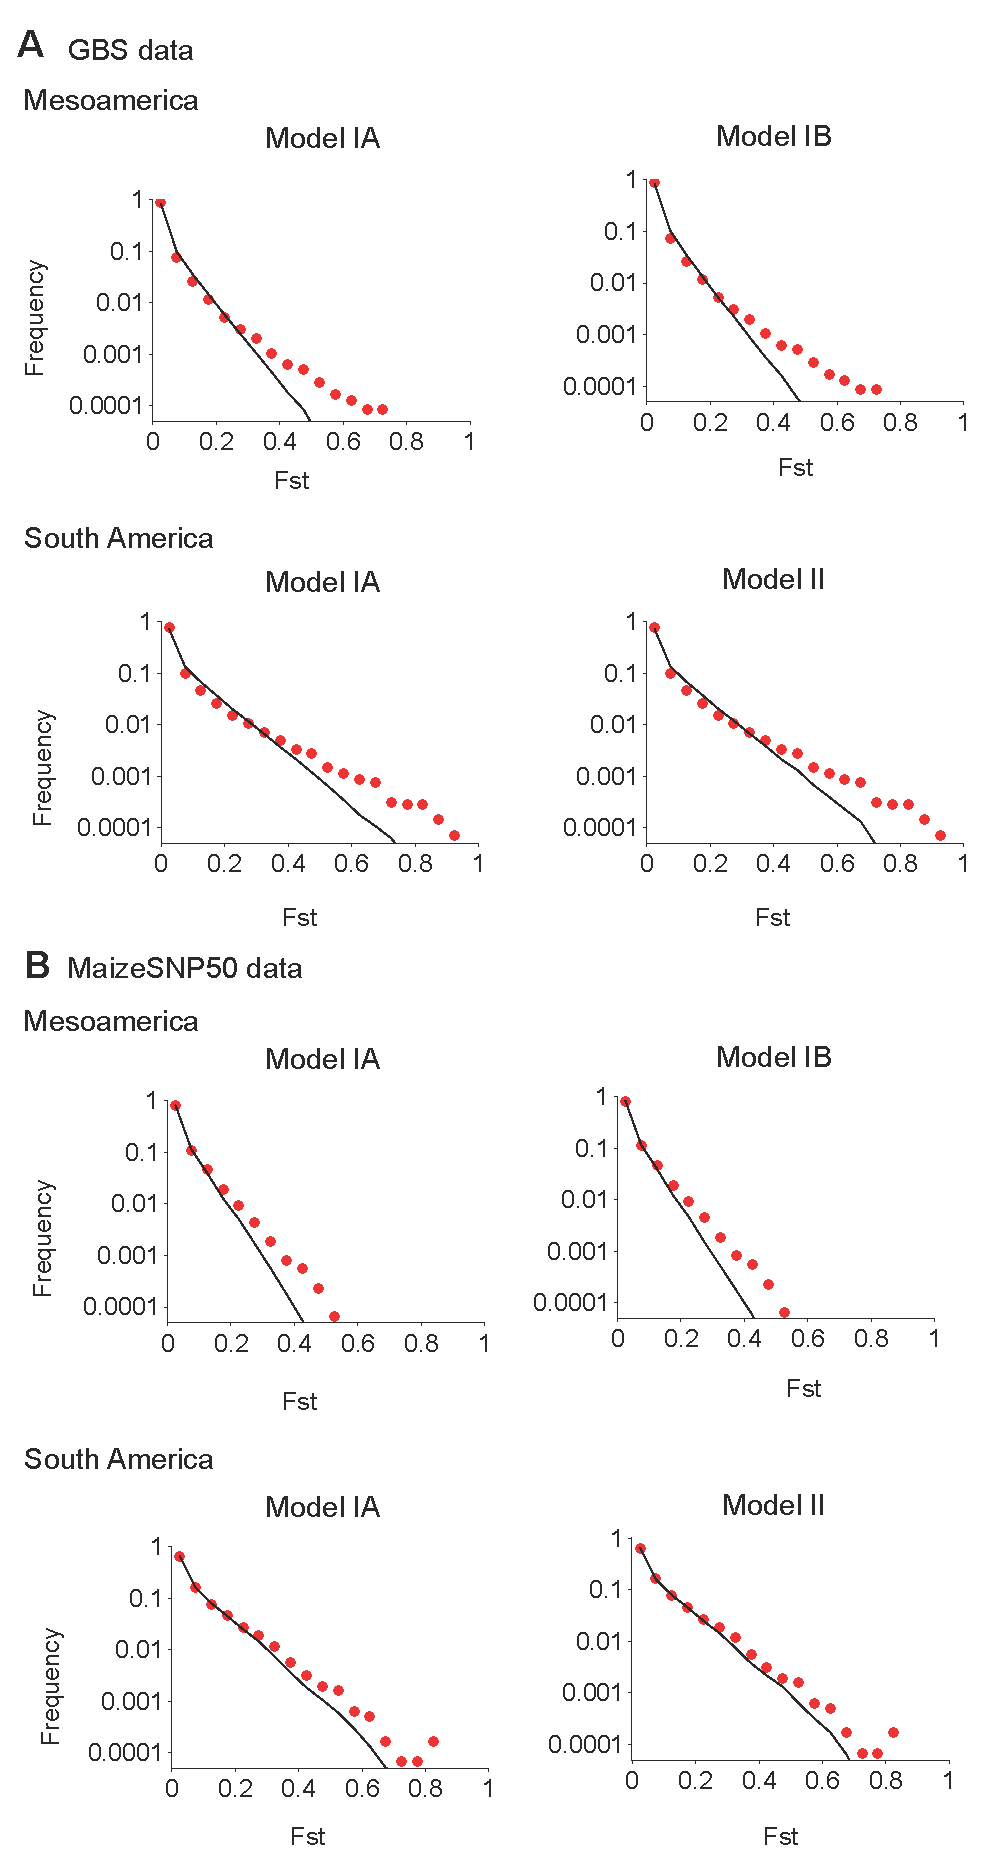
\includegraphics[width=0.45\textwidth]{fig/Fig5}
   \renewcommand{\baselinestretch}{0.9}
   \vspace{-3mm}
   \caption{Observed and expected distributions of $F_{ST}$ values in GBS (A) and MaizeSNP50 data (B).  The \emph{x}-axes represent $F_{ST}$ values.  The \emph{y}-axes represent the frequency of SNPs with $F_{ST}$ values within a bin of 0.05 size.  Red dots and solid lines indicate observed and expected distributions. 
   }
\vspace{-6mm}
    \label{FstDist}
  \end{center}
\end{figure}
%%%%%%%%%%%%%%%%%%%%%%%%%%%%%%%%%%%%%%%%%% FIGURE

%%%%%%%%%%%%%%%%%%%%%%%%%%%%%%%%%%%%%%%%%%%%%%%%%%%%%%%%%%%%
\begin{figure}[h]
  \begin{center}
    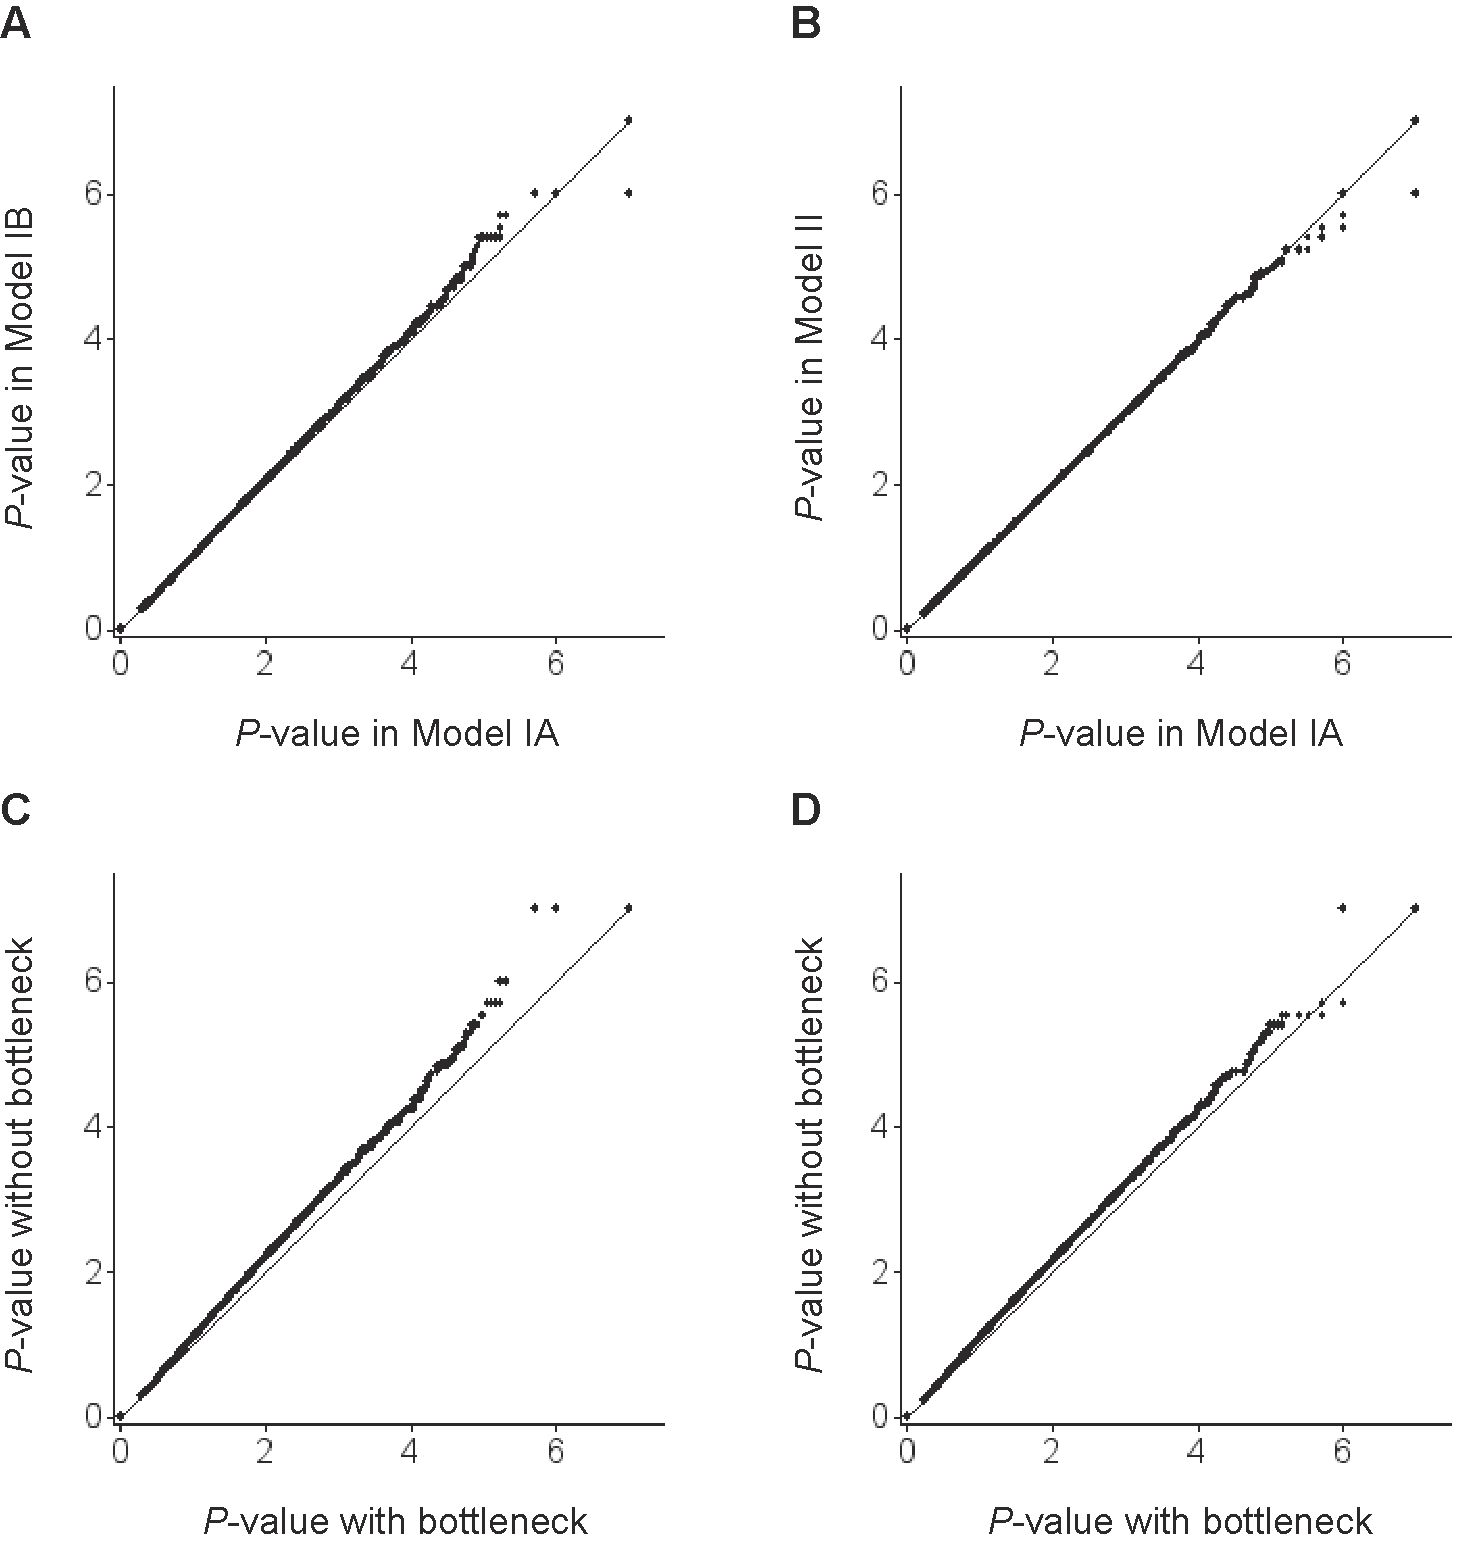
\includegraphics[width=0.6\columnwidth]{fig/bot2.pdf}
    \caption{Q-Q plot for $-$log$_{10}$-scaled \emph{P}-values of population differentiation between lowland and highland populations. (A) Model IA \emph{v.s.} Model IB in Mexico, (B) Model IA \emph{v.s.} Model II in S. America, (C) Model with \emph{v.s.} without bottleneck in Mexico and (D) Model with \emph{v.s.} without bottleneck in S. America.}
    \label{fig:qq}
  \end{center}
\end{figure}
%%%%%%%%%%%%%%%%%%%%%%%%%%%%%%%%%%%%%%%%%%%%%%%%%%%%%%%%%%%%



%%%%%%%%%%%%%%%%%%%%%%%%%%%%%%%%%%%%%%%%%%%%%%%%%%%%%%%%%%%%
\begin{figure}[h]
  \begin{center}
    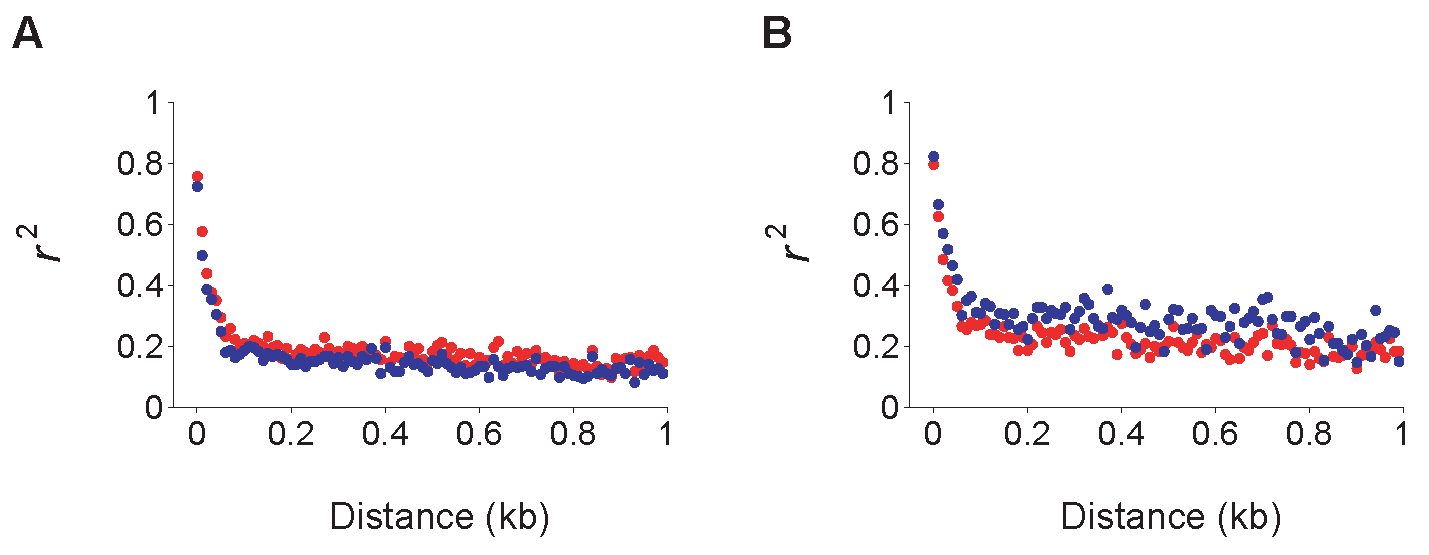
\includegraphics[width=0.7\columnwidth]{fig/LD.pdf}
    \caption{Pattern of decay of linkage equilibrium in Mexico (A) and South America (B).  Red and blue dots represent low- and highland population, respectively.  $r^2$ values were calculated as a statistics and averaged within 10-bp bins of distance between SNPs.  The \emph{x}- and \emph{y}-axes represent distance between SNPs (kb) and average $r^2$ values.}
    \label{supp:LD}
  \end{center}
\end{figure}
%%%%%%%%%%%%%%%%%%%%%%%%%%%%%%%%%%%%%%%%%%%%%%%%%%%%%%%%%%%%

\newpage
\suppl
\section*{File S1}

\section*{Directionality of adaptation} \label{sec:supptextsho}
%\noindent {\Large \textit{Text~S1} }

We classified the patterns of allelic differentiation among highland and lowland populations in Mexico and S. America together with the information of \emph{parviglumis} in an \emph{ad hoc} manner; the allelic differentiation pattern is consistent with highland or lowland adaptation scenario.  
In Figure~\ref{AllelePat}, we illustrate the frequency of putative ancestral and derived alleles in the five populations, drawn by red and blue, respectively.

First, we focus on the SNPs with the signature of adaptation only in Mexican populations (Figure~\ref{AllelePat}A).  
The first and second rows shows the typical patterns of highland adaptation with \emph{parviglumis} data available.
We simply assume that the allele in higher frequency in \emph{parviglumis} is ancestral.
%\jri{we have decent Tripsacum data now, should we go back and re-assess this?}

Both rows show the consistent pattern to highland adaptation in Mexico because the frequency of the putative derived allele in Mexican highlands is highly differentiated from those in both \emph{parviglumis} and Mexican lowlands.
The patterns in S. America are different between the first and second rows.
However, we do not take the patterns in S. American populations into account because there is no adaptive signature in S. American.
On the other hand, we should consider the allelic pattern in S. America in the case of the third row; we cannot utilize the information of \emph{parviglumis}.
It is impossible to infer the ancestral allele, so we assume the pattern is consistent with highland adaptation if one allele is in higher frequency in Mexican lowlands and S. American populations and the others is in higher frequency in Mexican highlands.
We classified the SNPs into lowland adaptation in the same way (from fourth to sixth rows in Figure~\ref{AllelePat}A).

Next, we consider the SNPs with the signatures of adaptation in both Mexico and S. America (Figure~\ref{AllelePat}B).
The pattern in the first row is consistent with parallel highland adaptation, whereas the second row shows parallel lowland adaptation. 
We cannot infer lowland or highland adaptation without the outgroup, so we ignore such SNPs.
The pattern in the third row is the special case: the allele frequency is similar between Mexican lowlands and S. American highlands and similar between Mexican highlands and S. American lowlands.
This pattern could be explained by that the SNP is linked to a read adaptive SNP and recombination breaks down the linkage between them.

Finally, we tested whether PHS test supports highland and lowland adaptation scenario.
Consider the case of highland adaptation.
We assumed that the putative derived allele is adaptive in highlands and checked whether the haplotype length is longer in highlands than that in lowlands.
However, haplotype length cannot be compared directly because the derived allele frequency is different between highlands and lowlands.
Thus, we compared the \emph{P}-values of PHS test as a indicator of haplotype length given allele frequency (Pr($PHS_{xA}\leq PHS_{null|p}$ in Materials and Methods).
We just say that the PHS test is consistent if the \emph{P}-value in highlands is smaller than the \emph{P}-value in lowlands (haplotype length is longer as \emph{P}-value is smaller).
The result is summarized in Table~S3.

\renewcommand{\thefigure}{\Roman{figure}}
\setcounter{figure}{0}

%%%%%%%%%%%%%%%%%%%%%%%%%%%%%%%%%%%%%%%%%%%%%%%%%%%%%%%%%%%%
\begin{figure}[b]
  \begin{center}
    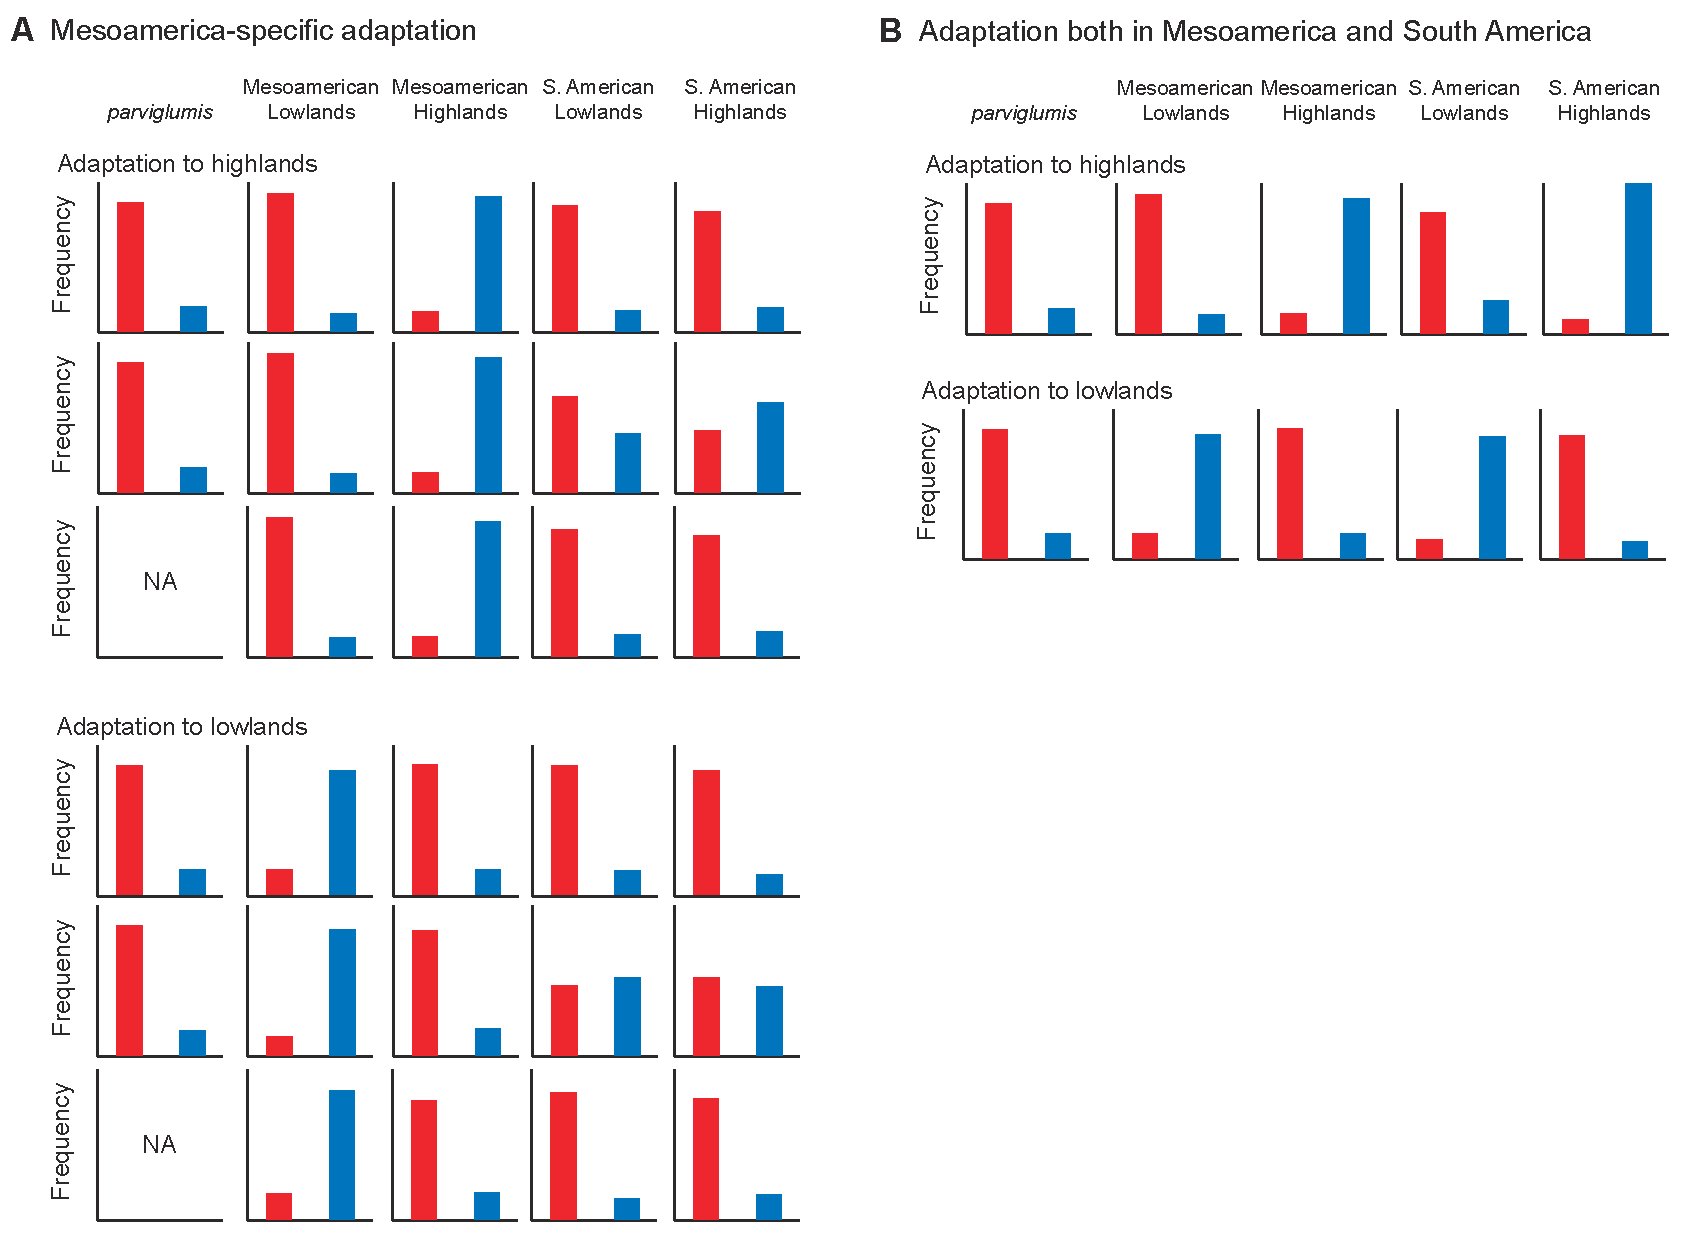
\includegraphics[width=0.9\columnwidth]{fig/AllelePat.pdf}
    \caption{Illustration of allele frequency changes in maize and \emph{parviglumis}.  Red and blue bars represent the allele frequency of ancestral and derived, adaptive alleles, respectively.  The allele frequencies in the five populations are shown: \emph{parviglumis}, Mexican lowlands and highlands, and S. America lowlands and highlands. NA in \emph{parviglumis} indicates that there is no SNP data in the site.}
    \label{AllelePat}
  \end{center}
\end{figure}
%%%%%%%%%%%%%%%%%%%%%%%%%%%%%%%%%%%%%%%%%%%%%%%%%%%%%%%%%%%%

















\end{document}

